\documentclass{article}

\usepackage{amsmath}
\usepackage{setspace}
\usepackage{xcolor}
\usepackage{graphicx}
\usepackage{subcaption}
\graphicspath{{figures/}}

\pagecolor{black}
\color{white}
\setcounter{section}{-1}

\title{Appunti per Metallurgia e Materiali non Metallici}
\date{19-02-2023}
\author{Matteo Sanderson}

\begin{document}

    \pagenumbering{gobble}
    \maketitle
    \newpage
    \setstretch{1.25}
    \newpage
    \tableofcontents
    \setcounter{tocdepth}{5}
    \newpage
    \pagenumbering{arabic}
    \section{Appunti iniziati}
        \subsection{Libri consigliati}
            \begin{itemize}
                \item Nicomedi - Metallurgia
                \item Nicomedi - Accai e leghe non ferrose
                \item Askeland - The Science and Engineering of Materials
                \item Campbell - Metallurgy and Engineering Alloys
            \end{itemize}
        I concetti sono importanti non le formule
        \subsection{Link}
            \begin{itemize}
                \item fa-fe.com
                \item fa-fe.it
                \item Password: 1141410931181
            \end{itemize}
        \subsection{Modalita' d'esame}
            Parte A (25\% del voto): Domande a risposta multipla. 2 punti per risposta corretta, 0 per nessuna risposta e -1 per risposta errata. Almeno 16 per passare.
            \newline Parte B (75\% del voto): Scritto a risposta aperta, 2 ore per 4 domande. Almeno 18 per passare.         
    \section{Lezione 1 - Introduzione}
            \subsection{Differenze tra metalli e leghe}
                I metalli, come ferro, alluminio, rame e nickel hanno delle leghe e il nome delle leghe gli e' stato dato o viene derivato dei metalli che creano la lega.
                L'accaio e' la lega piu' importante a cause delle sue proprieta' interessanti e il suo costo che e' relativamente basso.
                \newline    Una legha ferrosa con un contentuo minore di 2,11\% di carbonio e' nota come ferro invece una leghe ferrosa con un contenuto di carbonio maggiore di 2,11\% e' nota come ghisa.
                \newline    Ci sono anche leghe di alluminio e rame. Il rame crea leghe con altri metalli, la sua lega con lo stagno e' nota come il bronzo mentre la sua leghe con lo zinco e nota come l'ottone.
                \newline    Il titanio crea leghe ma sono fuori dello scopo del corso a causa dell'uso sparso a colpa del prezzo elevato del titanio.
            \subsection{Legami}
                \subsubsection{Legame Ionico/Ceramiche}
                    I legami ionici vengono creati a cause delle attrazione elettrostaticha tra anioni di non mettalli e cationi di metalli.
                    I legami ionici creano ceramiche. I materiali ceramici hanno molti usi anche in ambiti industriali tra piastrelle, sali e vetri.
                    Tutti i materiali ceramici sono sono composti da legami ionici.
                    \newline Esempi di materiali ceramici includono:
                    \begin{itemize}
                        \item Al\textsubscript{2}O\textsubscript{3} (Allumina)
                        \item SiO\textsubscript{2} (Silice)
                        \item NaCl 
                    \end{itemize}
                
                \subsubsection{Legame Covalente/Polimeri}
                    I polimeri(organici) sono creati da numeri grandi di monomeri, che catene lunghe di carbonio.
                    I polimeri possono esser visti come degli spaghetti, dove se non ci metti l'olio dopo essere cotti possono avere delle proprieta diverse.
                    \newline \newline I polimeri termoplastici sono polimeri che dopo essere formati possono essere ririscaldati per dargli una nuova forma,
                    questo e' perche i materiali sono solo tenuti insieme da legami idrogeni e altri legami deboli che possono riformarsi se rotti.
                    Invece i polimeri termodurenti sono polimeri che quando gli viene data un forma non puo' essere piu' cambiata, questo
                    e' a cause delle retticolazione (cross-linking), che e' un effetto dove i monomeri creano legami covalenti tramite i gruppi funzionali che
                    non possono esser rotti facilmente percio' i polimeri termodurenti di solito bruciano prima di sciogliersi.

                \subsubsection{Legame Metallico}
                    In un legame metallico tutti gli atomi perdono i loro elettroni di valenza e essi vanno nella nube di elettroni che charatterizza un legame metallico.
                    Gli atomi percio' hanno carica positiva mentre la nube ha carica negativa, questo crea una attrazione elettrostatica che mantiene il materiale insieme.
                    \newline Gli atomi si mettono in una retticola a distanze costanti a cause di forze di attrazione e repulsione che ci sono fra gl'atomi e gl'atomi e gl'atomi e la nube di elettroni.
            
            \subsection{Caratterristiche importanti dei legami}
                \hangindent=0.7cm \textbf{Caratteristica importante delle ceramiche:}
                \newline \hangindent=0.7cm Le caratteristiche degli elementi componenti sono perse nelle ceramiche e il materiali guadagna proprieta' sue.
                \newline \newline \textbf{Caratteristica importante dei polimeri:}
                \newline Anche i monomeri perdono le proprieta' degli elementi che li compongono.
                \newline \newline \textbf{Caratteristiche importanti dei composti metallici:}
                \begin{itemize}
                    \item Elevata energia e forza di legame
                    \item Comportamento isotopo (assenza di prorieta' direzionali [come in ceramiche e polimeri])
                    \item Assenza localizzazione della carica elettrica
                    \item Conduttivita' elettrica e termica $\longrightarrow $ Perche elettroni non sono bloccati e invece sono liberi di muoversi influenzare l'un l'altro.
                    \item Alta lucentezza $\longrightarrow $ I fotoni che colpiscono la superfice colpiscono gli elettroni nella nube e vengono assorbiti e sparati indietro(diagrammi Feynman).
                    \item Alta compattezza e densita'
                \end{itemize}

            \subsection{Caratteristica fondamentale dei metalli}
                Tutte le classi di materiali (ceramiche, polimieri e metalli) possono essere deformati plasticamente,
                pero i metalli sono gli unici che possono essere deformati plasticamente senza rompersi.
                \newline \newline La deformazione plastica e' definita da uno scorrimento degl'atomi in una struttura.
                \newline \newline I metalli sono gli unici che possono deformarsi senza rompersi perche la struttura dei metalli non dipende dalla posizione specifica di cariche,
                come nei legami ionici, percio' quando c'e' uno scorrimento gli elettroni mantengono la struttura mentre gli atomi cambiano solo gli atomi sui hanno effetto la loro repulsione.
                \newline \newline Se lo scorrimento occorresse in un retticolo ionico gli anioni e cationi si incontrerebbero e ci sarebbe un repulsione percio' si romperebbe.
                \newline \newline Invece nei polimeri la ragioni sono diverse. Nei polimeri termoplastici con uno scorrimento i legami ad idrogeno si rompono e gli monomeri si muovono,
                 questo puo essere visto un sacchetto che si stira e poi si rompe. Se si tentasse di deformare i monomeri se stessi i monomeri si deformerebbero elasticamente e con abbastanza
                 forza i legami covalenti del monomero si romperebbero. In un polimero termodurente, la deformazione plastica non occorre perche la struttura e' un retticolo grande e percio'
                 si possono solo rompere i legami covalenti percio' cambiando la struttura effettiva.
                 \newline \newline A causa di queste proprieta la ceramiche e i polimieri possono essere chiamati \textcolor{red}{\textbf{Fragili}}. Fragile significa che non occorre deformazione plastica prima
                 che il materiale si rompa. Invece i metalli sono chiamati \textcolor{red}{\textbf{Duttili}}. Duttile significa che dopo abbastanza deformazione plastica il materiale si rompe. La deformazione
                 plastica e' progressiva prima di rompersi, questo e' importante perche' in casi industriali si possono vedere deformazione dei metalli prima che si rompa, percio' e' piu' sicuro.
    \newpage
    \section{Lezione 2 - Retticoli cristallini dei metalli}
        \begin{figure}[h!]
            \centering
            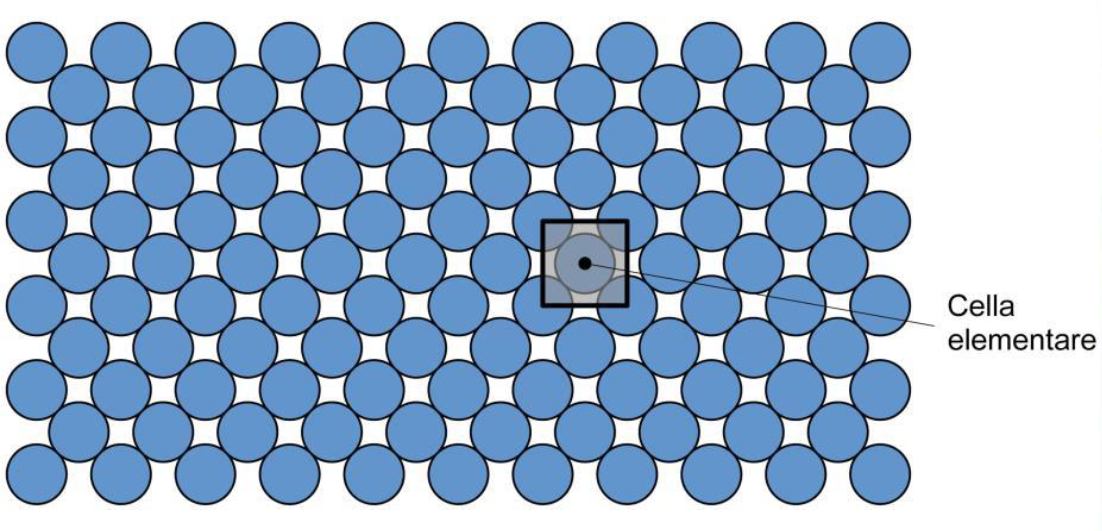
\includegraphics[width=\linewidth]{Retticolo pre 1800.png}
            \caption{Retticolo cristallino dei metalli alla fine dell'1800}
        \end{figure}
        La figura fa vedere l'idea che gli scienziati alla fine del 1800 avevano sulla struttura del retticolo metallico.
        Oltra la ovvia mancanza della nube di elettroni, l'idea e' per la maggior parte la struttura e' giusta.
        \newline \newline La metallurgia spiega le proprieta' macroscopiche con la proprieta' microscopiche del materiale.

        In generale per i materiali metallici piu' deformabile il materiale meno e' rigido e meno e' deformabile piu' e' resistente.

        I materiali mettalici sono disposti in modo regolare noto come un retticolo, questo retticolo e'
         composti da celle elementari che si ripetono e creano il retticolo grande nel metallo.

        \newpage
        \subsection{Tipi di celle elementari}
            \subsubsection{Reticolo cubico a corpo centrato (CCC)}
                \begin{figure}[h!]
                    \centering
                    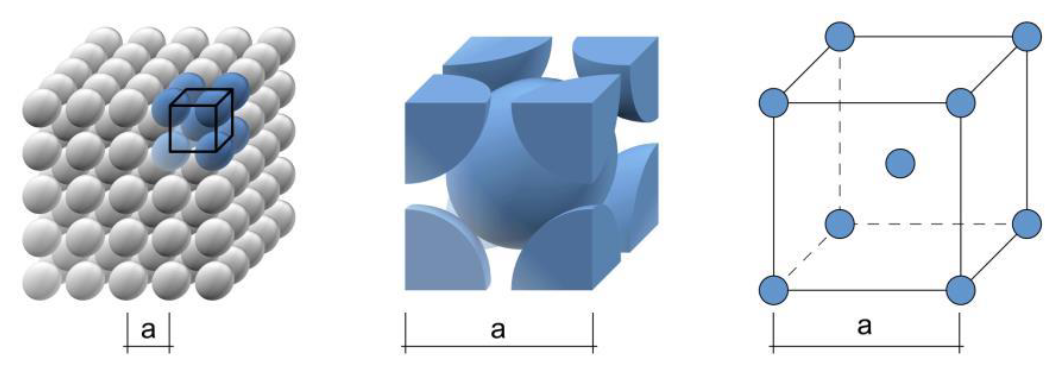
\includegraphics[width=\linewidth]{Reticolo cubico a corpo centrato.png}
                \end{figure}
                In un reticolo cubico a corpo centrato un atomo e' centrato nella cella con altri altri atomi posti ad ogni vertice che comprende l'atomo centrale.
                Gli atomi si toccano lungo la diagonale del cubo.
                \newline \newline Questa strutture per le celle elementari e' usata dal cromio(Cr), vanadio(V), tungsteno(W), molibdeno(Mo), litio(Li), sodio(Na) e calcio(Ca), e' anche
                la struttura del ferro(Fe) quando $T<912^o C$ e quando $1396^o C<T<1538^o C$.
                \newline \newline Il ferro e' un materiale allotropico, che significa che subisce una trasformazione che cambia la forma delle sue celle elementari.
                \newline \newline Il reticolo CCC a due atomi propri che lo compongono.
                \begin{figure}[h!]
                    \centering
                    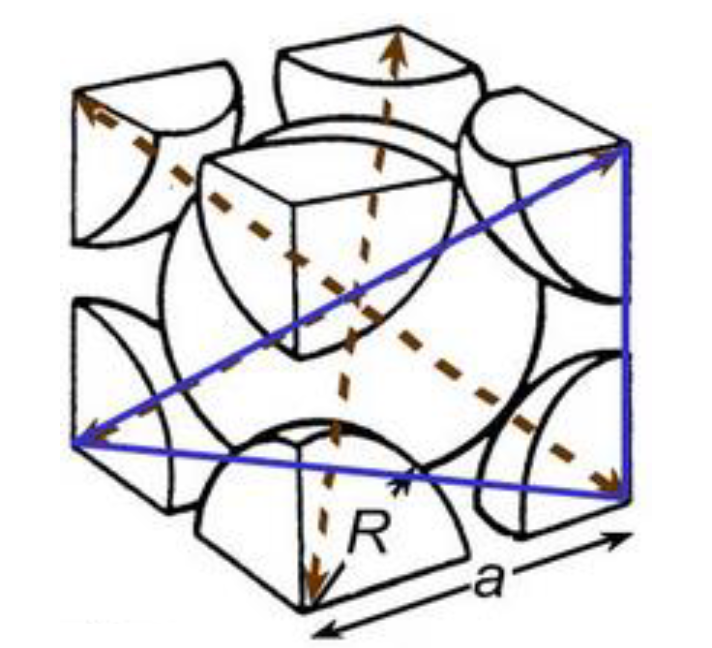
\includegraphics[width=0.5\linewidth]{CCC calcolo}
                \end{figure}
                \begin{gather}
                    (4R)^2 = a^2 + (a \sqrt{2})^2 \\
                    a = \frac{4R}{\sqrt{3}} \label{CCC_reference} \\
                    a^3 = 12,32 R^3
                \end{gather}

            \subsubsection{Fattori di compattazione atomica (APF - Atomic Packing Factor) per il reticolo CCC}
                \paragraph{Definizione di APF} L'APF e' usato per determinare la densita di una cella elementare o potrebbe esser visto come la percentuale del volume in una cella e' occupata da atomi. 
                \begin{equation}
                    APF = \frac{\text{Volume degli atomi nella cella}}{\text{Volume nella cella}}
                \end{equation}
                \begin{gather}
                    V_\text{atomi} = 2 * \frac{4}{3} \pi R^3 \cong 8,37 R^3 \\
                    V_\text{cella} \cong 12,32 R^3 \\
                    APF_\text{CCC} = \frac{V_\text{atomi}}{V_\text{cella}} = \frac{8,37 R^3}{12,32 R^3} \cong 0,68
                \end{gather}

                $\Longrightarrow$ Il volume del reticolo CCC e' occupato il 68\% da atomi.
            
            \subsubsection{Reticolo cubico a facce centrate (CFC)}
                \begin{figure}[h!]
                    \centering
                    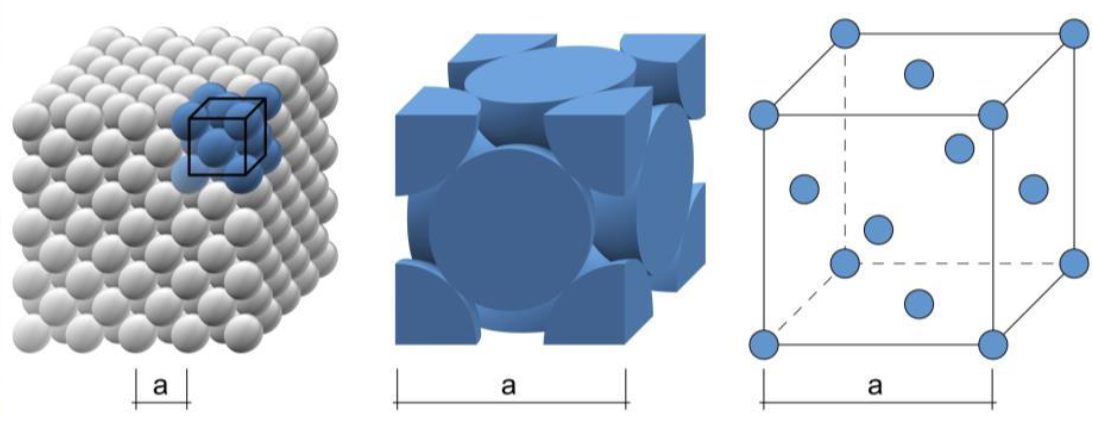
\includegraphics[width=\linewidth]{Reticolo CFC}
                \end{figure}
                Il reticolo CFC e' una struttura piu' complessa del reticolo CCC, questo e' perche il reticolo CFC ha le facce che puntano verso il centro non ha un atomo centrale.
                Questo significa che ci sono 4 atomi propri nel reticolo CFC invece dei 2 del reticolo CCC, e causa il volume del reticolo CFC ad esser piu' grande del reticolo CCC perche 
                la tangenza degli atomi occorrere sulla diagonale delle facce della cella in confronto con la diagonale del cubo intero come nei reticolo CCC.
                \newline \newline Il reticolo CFC e' il reticolo usato dal rame(Cu), argento (Ag), oro (Au), alluminio (Al), nickel(Ni), piombo (Pb), platino(Pt) e 
                il ferro quando $912^o C<T<1396^o C$.
                \newline \newline Tutti i metalli elencati sono noti per la loro deformabilita', quindi si puo' capire il reticolo e' la cause della deformabilita'.
                \newline \newline Il ferro quando entra questa forma diventa piu' maleabile/deformabile, questo spiega perche' i fabbri ferrai riscaldano il ferro 
                prima di colpirlo.
                \begin{figure}[h!]
                    \centering
                    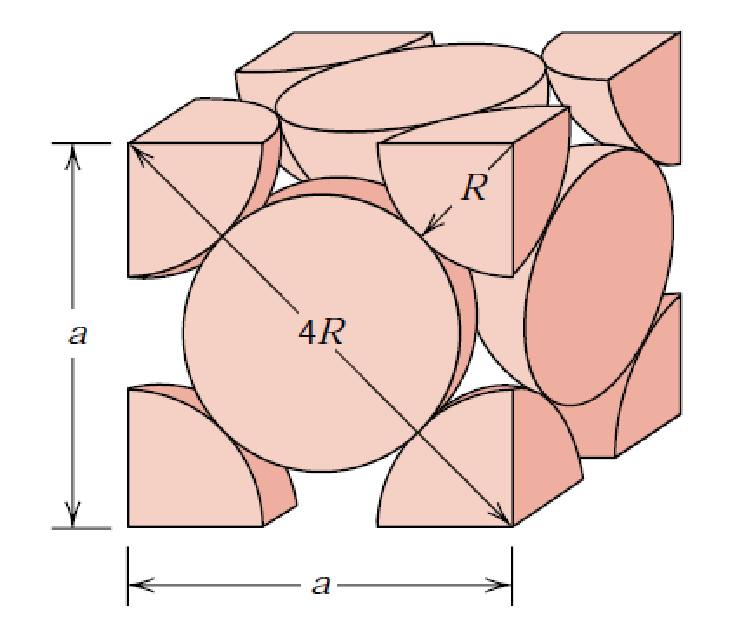
\includegraphics[width=.5\linewidth]{CFC calcolo}
                \end{figure}
                \begin{gather}
                    (4R)^2 = a^2 + a^2 \\
                    a = \frac{4}{\sqrt{2}} R \label{CFC_reference}\\
                    a^3 \cong 22,63 R^3
                \end{gather}
                Il fatto che la lunghezza dei lati $a$ nel reticolo CCC (\ref{CCC_reference}) e' piu' piccolo di $a$ nel reticolo CFC 
                (\ref{CFC_reference}) spiega matematicamente perche' il reticolo CFC e' piu' voluminoso del retiolo CCC.
            \subsubsection{Fattori di compattizione atomica (APF) per il reticolo CFC}
                \begin{gather}
                    V_\text{atomi} = 4 * \frac{4}{3} \pi  R^3 \cong 16,76 R^3 \\
                    V_\text{cella} \cong 22,63 \\
                    APF_\text{CFC} = \frac{V_\text{atomi}}{V_\text{cella}} = \frac{16,76 R^3}{22,63 R^3} \cong 0,74
                \end{gather}
                $\Longrightarrow$ Il volume del reticolo CFC e' occupato il 68\% da atomi.

            \subsection{Regione per il cambio di deformabilita'}
                La deformabilita' e' causata dalla quantita' di spazio che e' vuota (spazio vuoto si chiama anche lacuna).
                Il reticolo CFC e' piu' deformabile del reticolo CCC perche' anche se ha piu' spazio occupato occupato da atomi (74\%) in confronto al reticolo CCC (68\%), 
                il reticolo CFC e' piu' voluminoso quindi la percentuale piu' piccola di lacune nel reticolo CFC e' piu' grande della percentuale piu' grande del reticolo piu' piccolo.
                Le leghe sono create mettendo atomi di altri elementi nelle lacune. I metalli con il reticolo CFC formano leghe piu' prevalentamente per questa ragione.
        \subsection{Fasi strutturali del ferro}
            \begin{figure}[h!]
                \centering
                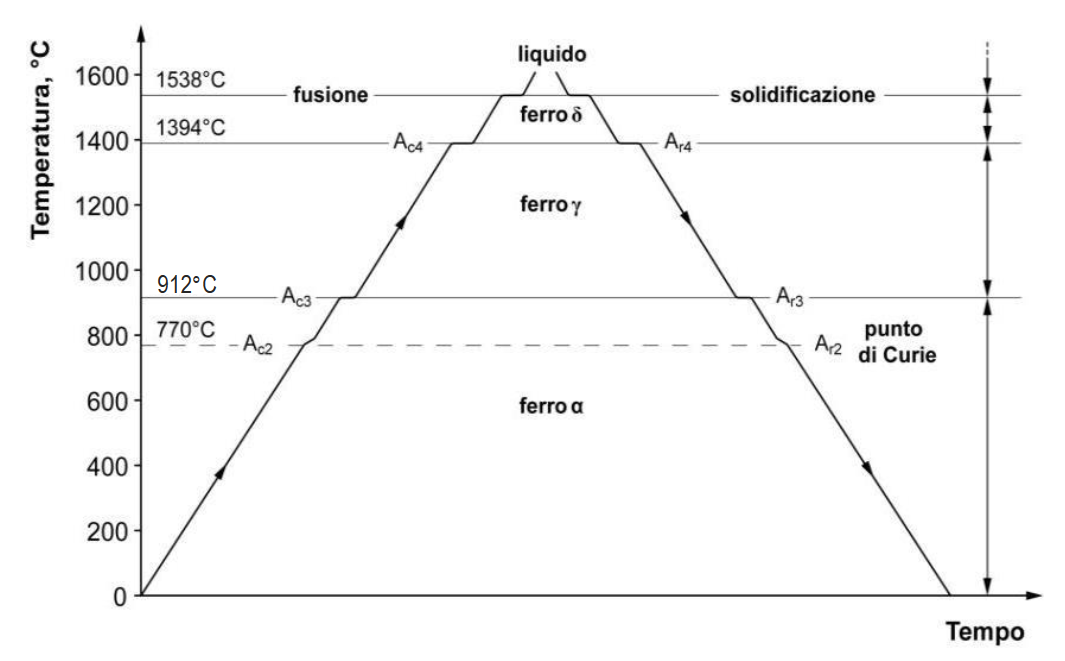
\includegraphics[width=.85\linewidth]{Fasi Ferro.png}
                \end{figure}
            Come cennato prima, il ferro e' un materiale allotropico che significa che cambia forma retticolare al cambio della temperatura.
            Il ferro ha tre fasi retticolari note come $\alpha$ , $\gamma$ e $\delta$. $\alpha$ e $\delta$ sono fasi dove il ferro ha una reticolo CCC 
            invece la nella fase $\gamma$ il ferro ha un reticolo CFC. $\alpha$ e $\delta$ sono chiamati diversamente per facilitare la identificazione 
            della temperatura.
            \newline \newline Gli scalini (punti critici, notati da A\textsubscript{cn} e A\textsubscript{rn}), occorrono quando c'e' un cambio nel 
            ferro in cui c'e' bisogno di energia per effettuarlo.
            \newline \newline Un punto critico nella struttura (A\textsubscript{c2} e A\textsubscript{r2}) e' il "Punto di Curie", questo non 
            occorre quando la struttura del ferro cambia invece a questa temperatura il ferro perde il suo ferromagnetismo e diventa amagnetico.
            \begin{figure}[h!]
                \centering
                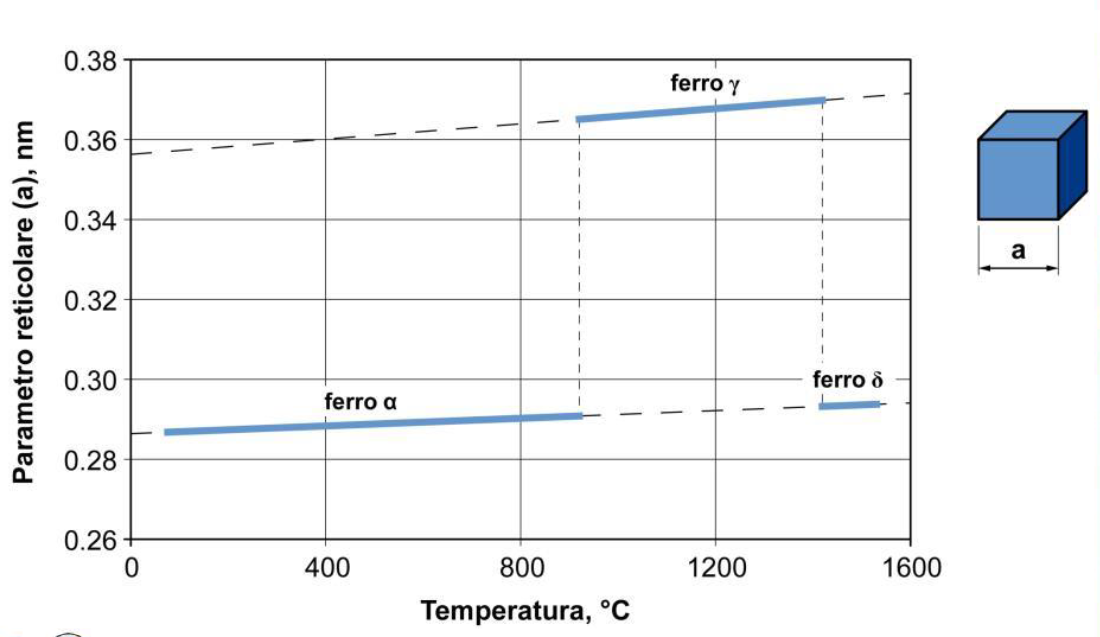
\includegraphics[width=.85\linewidth]{Cambio parametro reticolare nel ferro.png}
            \end{figure} 
            Questa figure mette in evidenza il cambio del parametro reticolare, cioe' la lunghezza di un lato di una celle elementare, nel ferro 
            con il cambio della temperatura e con se il cambio della struttura reticolare.
    \newpage
    \section{Lezione 3 - Reticoli, e diffetti e i loro positivi}    
        \subsection{Reticolo esagonale compatto (HCP)}
            \begin{figure}[ht!]
                \centering
                \begin{subfigure}{.25\linewidth}
                    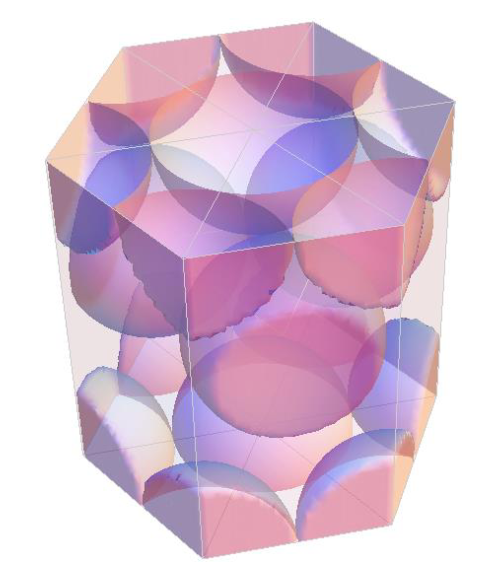
\includegraphics[width=\linewidth]{HCP grafico.png}
                \end{subfigure}
                \begin{subfigure}{.65\linewidth}
                    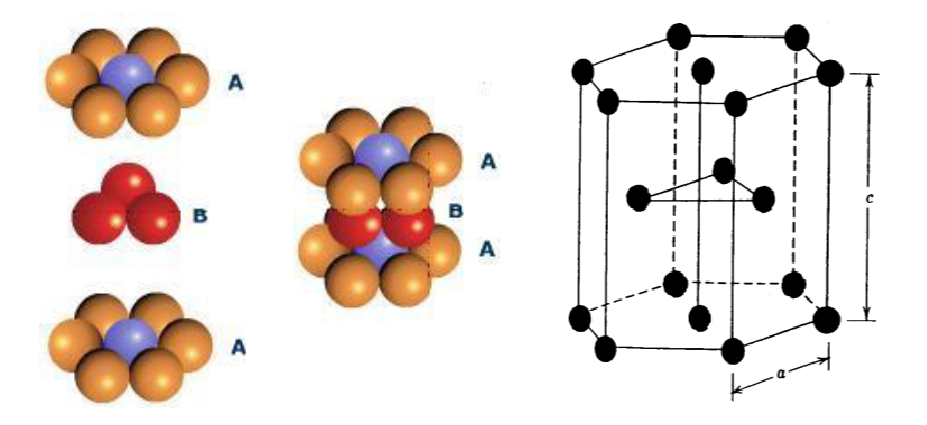
\includegraphics[width=\linewidth]{HCP schematica.png}
                \end{subfigure}
            \end{figure}
            Il reticolo esagonale compatto (HCP) e' usato dal titanio quando $T<882^o C$, dal magnesio, lo zinco, il cadmio e il cobalto. 
            Questi metalli sono resistenti ma \textcolor{red}{fragili} (fragile = tendenza a rompersi come il vetro). Aggiunto al costo piu' basso, l'accaio e' meglio del titanio 
            perche' a piu' \textcolor{red}{tenace} (tenace opposto di fragile).
            \newline \newline Il HCP ha un APF $=0,74$ ed e' composto da 6 atomi propri.

        \subsection{Difetti dei reticoli}
        Ogni reticolo contiene difetti perche' niente e' perfetto, i difetti nei reticolo sono (per la maggior parte) positivi e aiutano con delle 
        proprita dei metalli.
            \subsubsection{Difetti di punto}
                \paragraph{Vacanza} \mbox{}\\
                Una vacanza e' quando c'e' una mancanza di atomi in un certo punto, che cause la compressione degli atomi circostanti a causa di forze repulsiv piu' 
                deboli di se ci fosse un altro atomo.
                \paragraph{Atomi sostituzionali} \mbox{} \\
                Un atomo sostituzionale e' un atomo di una altro elemento che sostituisce un atomo del elemento principale. Questo e' uno dei due metodi per createre 
                le leghe, quindi tecnicamente le leghe sono metalli con difetti.
                \newline \newline Un esempio di una lega creata da atomi sostituzionali e' l'otone che creato da 60\% rame e 40\% zinco.
                \begin{figure}[ht]
                    \centering
                    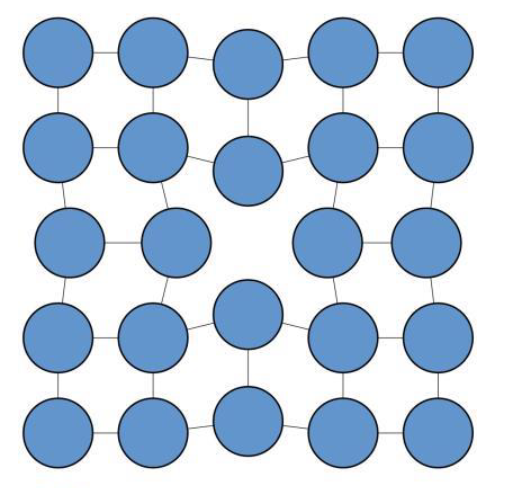
\includegraphics[width=.5\linewidth]{Vacanze.png}
                    \caption{Diagramma semplice di una vacanza reticolare.}
                \end{figure}
                \begin{figure}[ht]
                    \centering
                    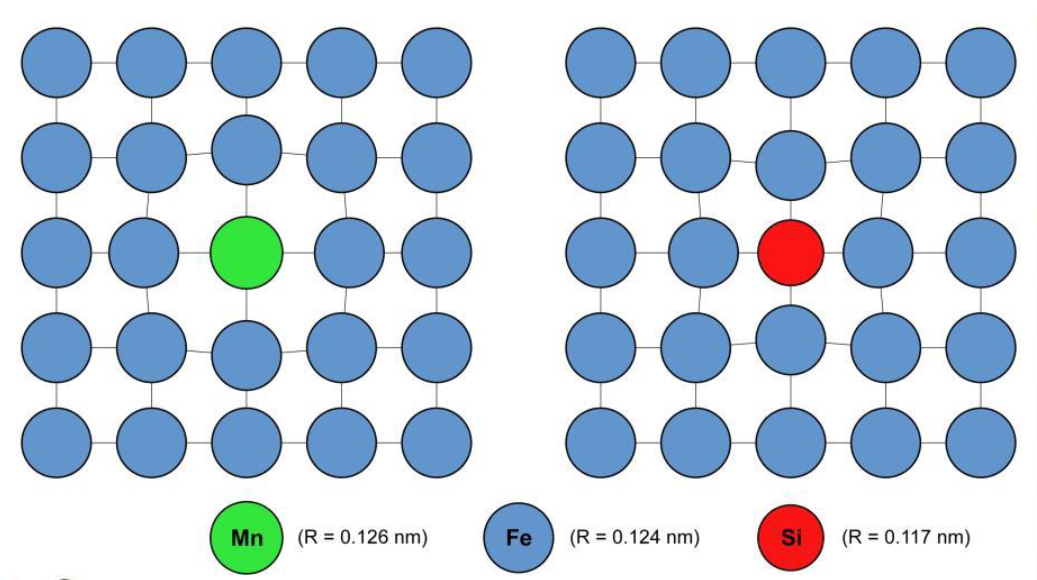
\includegraphics[width=.85\linewidth]{Sostituzione.png}
                \end{figure}
                \newline \newline Nella sostituzione gli atomi che sostituiscono devono essere di dimensioni simili all'atomo principale, se sono troppo grandi i due elementi non sono solubili, 
                e quindi non si crea una lega. Se gli atomi sono di dimensione simile la struttura cambia in corrispondenza alla dimensione dell'atomo sostituente. Se l'atomo e' piu' grande 
                dell'atomo principale, il reticolo circostante si espande a cause di forze repulsive piu' forti, mentre se il diametro e' piu' piccole dell'atomo originale, il reticolo 
                ciscostante si restringe a cause di forze repulsive piu' deboli.
                \paragraph{Atomi interstiziali}\mbox \\
                Un atomo interstiziale e' un atomo decisamente piu' piccolo degli atomi dell'elemento originale che si mette nei buchi del reticolo e cause distrubi alle struttura. Questi 
                disturbi sono piu' grandi dei disturbi che sono creati dagli atomi sostituzionali, qui gli atomi interseziali hanno un effetto piu' grande sulla resistenza di un reticoli 
                che gli atomi sostituzionali.
                \begin{figure}[ht]
                    \centering
                    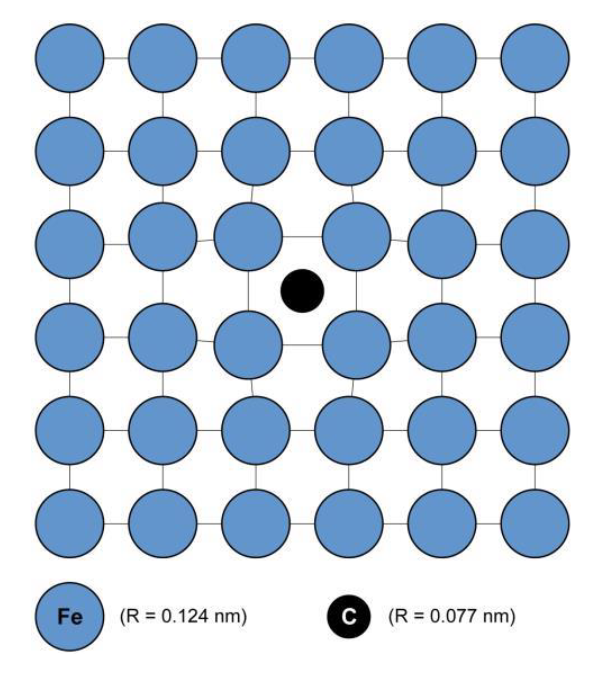
\includegraphics[width=.85\linewidth]{Interstiziali.png}
                \end{figure}
                Un combinazione di atomi sostituzionali e interstiziali e' la cosa migliore per creare un reticolo resistente.
        \subsection{Leghe vs. Metalli Puri}
            Le leghe sono piu' resistenti alle deformazioni a cause dei loro difetti, i difetti causano disturbi al reticolo che lo rendono piu' resistenti alle deformazione.
            Questo disturbi occorro nella forma di una perturbazione del campo elettromagnetico nel retticolo e per cio' la resistenza aumenta.
            \begin{figure}[ht]
                \centering
                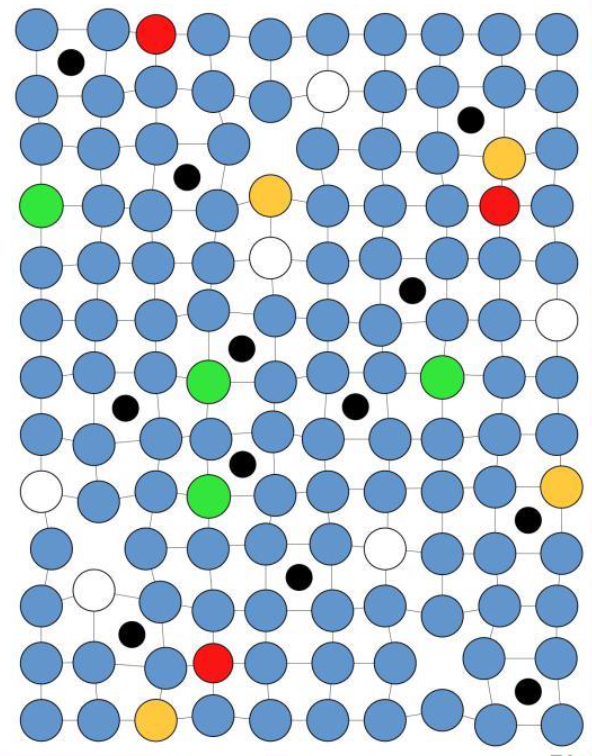
\includegraphics[width=.75\linewidth]{Reticolo Accaio.png}
            \end{figure}
            Nella figure si vede un diagramma del reticolo d'accaio (non esatto), questo rappresenta il fatto che l'accaio e' una lega base ferro e carbonio, ma contiene anche molti 
            altri elementi che cambiano se stessi la struttura.
        \subsection{Rafforzamento per soluzione solida/rafforzamento per alligazione (creare una lega metallica)}
            \begin{figure}[ht]
                \centering
                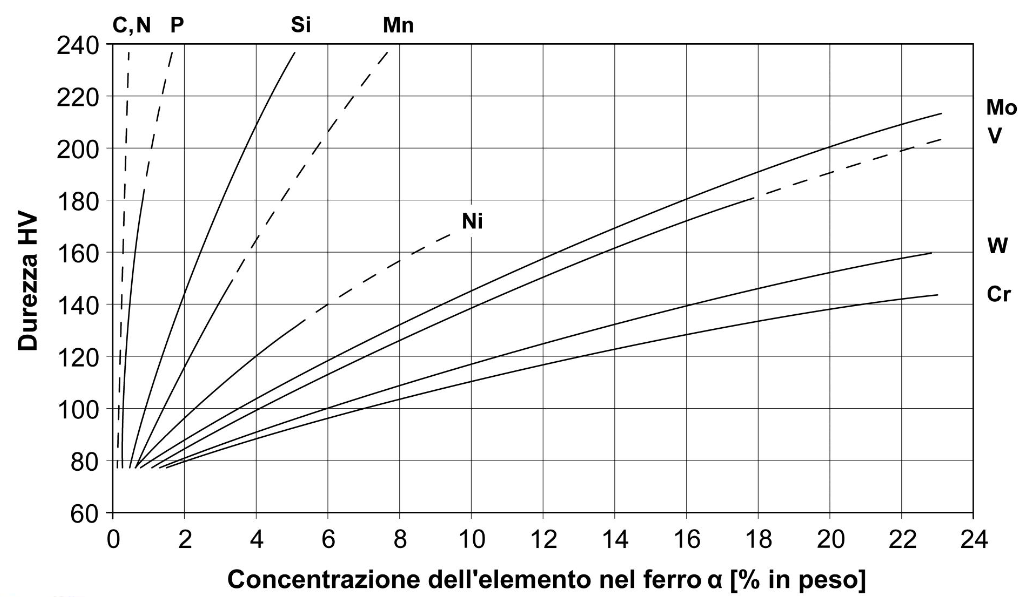
\includegraphics[width=.85\linewidth]{Rafforzamento per soluzione solida.png}
            \end{figure}
            Il diagramma rappresenta la quantita di certi elementi che devono essere aggiunti al ferro per aumentare la durezza di una certa quantita'.
            Quello che possiamo vedere e' che il carbonio e azoto, che sono atomi interstiziali per il ferro aumentano la durezza con una concentrazione 
            molto bassa invece altri metalli che sono atomi sostituzionali per il ferro hanno un effetto piu' basso con concentrazioni piu' elevate, questo 
            di nuovo rafforza l'idea che gli atomi interstiziali hanno un effetto grande sulla resistenza delle leghe.
        \subsection{Reticolo cristallino disordinato/ordinato}
            I reticoli disordinati sono piu' resistenti dei reticoli ordinati.
            \begin{figure}[ht]
                \centering
                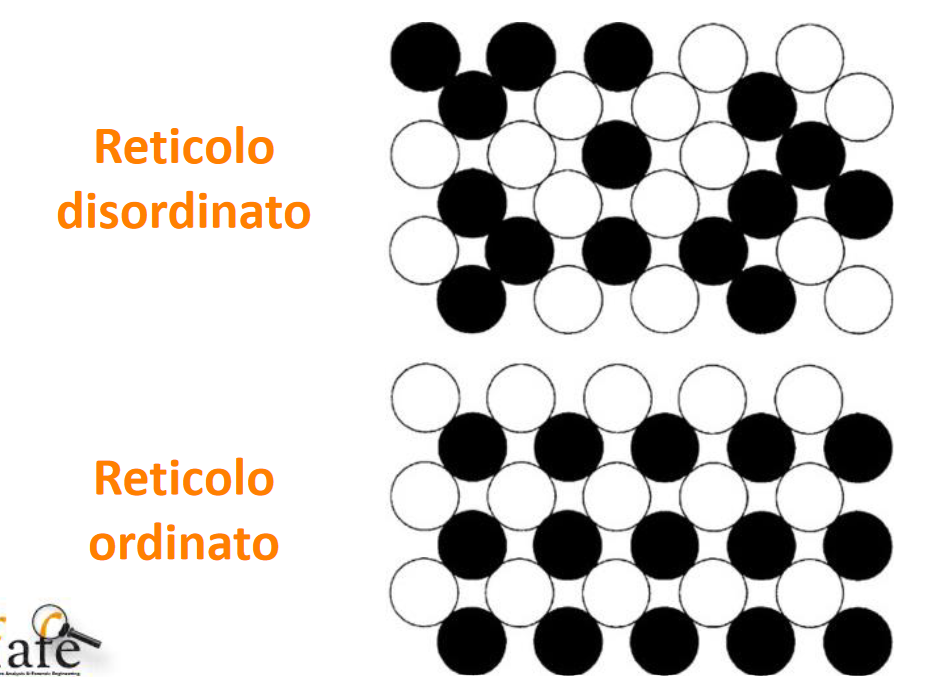
\includegraphics[width=.75\linewidth]{Disordinato Ordinato.png}
            \end{figure}
        \subsection{Solubilita' tra elementi e composti}
        Gli elementi hanno diverse compabilita' con l'un l'altro, alcuni elementi si mischiano bene ad ogni temperatura. Alcuni elementi non si mischiano 
        molto e estiste un limite alla loro solubilita' e se il limite e' passato non si mischiano piu', mentre alcuni elementi non si mischiano a qualsiasi temperature.
        Questo effetto si piu' spiegare con gli atomi sostituzionali e interstiziali. Come detto prima negli atomi atomi sostituzionali, se gli atomi hanno dimensioni 
        troppo diverse non si mischiano, invence con gli atomi interstiziali si crea il limite perche' causano troppi disturbo al reticolo del materiale e quindi troppo 
        causerebbe una deformazione del reticolo.
        \begin{figure}
            \centering
            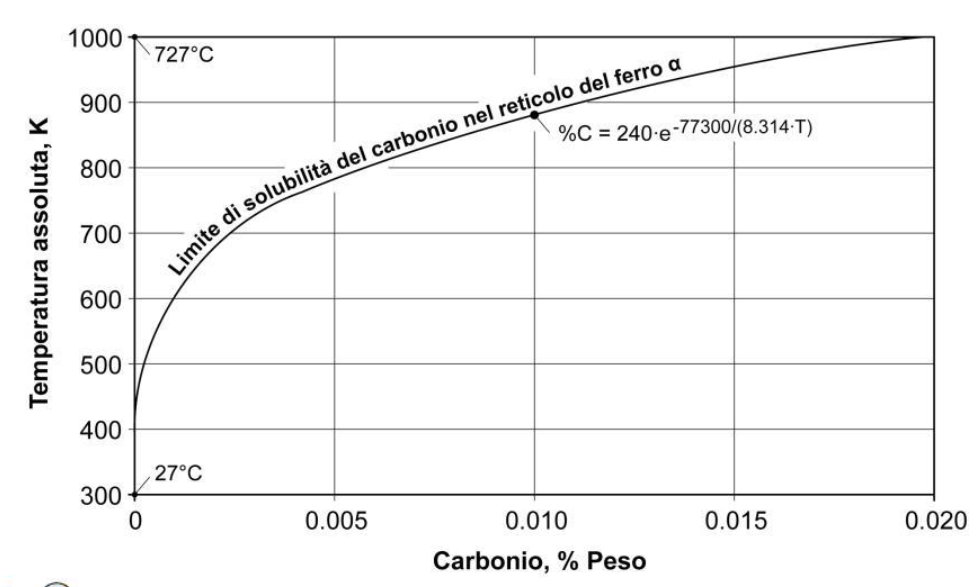
\includegraphics[width=.85\linewidth]{Solubilita'.png}
            \caption{Questo grafico rappresenta la linea del limite di solubilita' tra il carbonio e il ferro e spiega perche ci si mette cosi poco carbonio nell'accaio.}
        \end{figure}
        \newline \newline Ci sono 4 classi di rapporti nella solubilita' di elementi, gli elementi possono:
        \begin{itemize}
            \item Avere perfetta solubilita' (Ag e Au)
            \item Avere parziale solubilta' (Fe e C)(Limite)
            \item Avere perfetta insolubilta' (Fe Pb)
        \end{itemize}
        \subsubsection{Composti Chimici}
            La quarta possibilita' di solubilita' tra 2 elementi e' che creino un composto chimico invece di mischiarsi.
            Per esempi il Fe o O, che quando mischiati creano FeO, un composto ionico.
            I composti possono non avere niente a che fare con il composto e sono completamente inglobati dal reticolo. 
            Le dimensioni interatomiche nel composto sono di solito simili a quelle del reticolo che lo inglobano.
            \newline \newline I composti vengono in due tipi, i composti coerenti e i composti incoerenti.
            \begin{figure}
                \centering
                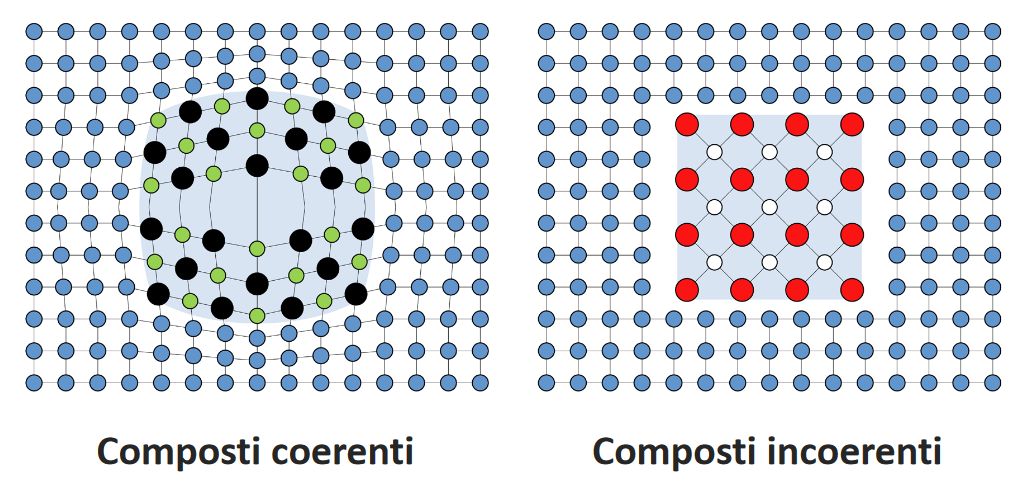
\includegraphics[width=.85\linewidth]{Tipi di Composti.png}
            \end{figure}
            La coerenza ha a che fare con l'orientamento del composto in confronto al reticolo. I composti coerenti, hanno un orientamento che e' uguale a quella del 
            reticolo inglobante e questo permette al composto di creare legami con il reticolo, invece in composti incoerenti il composto un orientamento diverso dal 
            reticolo inglobante per cio' il composto non puo' creare legami con il reticolo inglobante.
    \section{Lezione 4 - Altri difetti e Rafforzamenti}
        \subsection{Difetti di Linea}
            \subsubsection{Difetti di Linea/Dislocazione a spigolo}
                La \underline{\textbf{Dislocazione a spigolo}} \'e l'unico diffeto di linea di cui parleremo, anche se tanti altri esistono.\\
                Una dislocazione a spigolo \'e una mancanza di un semipiano cristallino grafico. Pu\'o esser visto come strappare a met\'a una pagine e chiudere il libro, le pagine solo si piegano per riempire il posto come ci sarebbe la parte che \'e stata rimossa. Viene chiamato diffetto di linea perch\'e la dislocazione non occorre solo in un punto ma lungo tutto il piano difettivo lungo una linea (la fine del piano) che esce ed entra dalla pagina.
                \begin{figure}[h!]
                    \centering
                    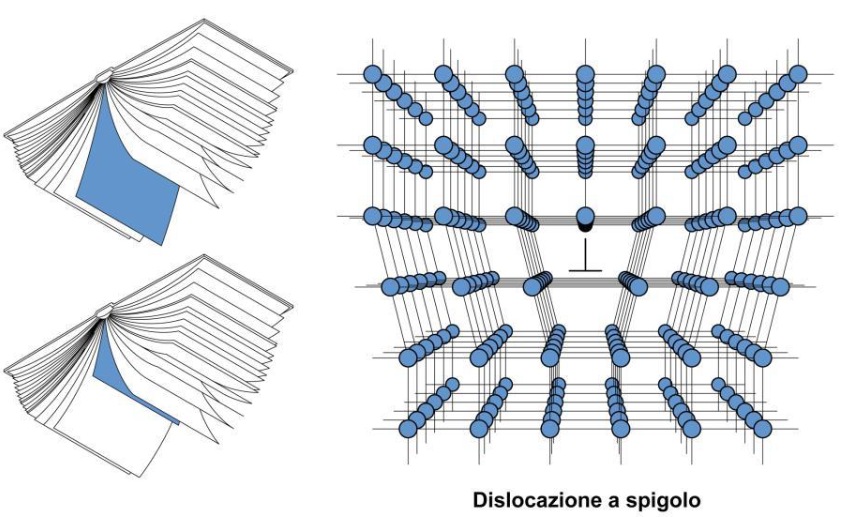
\includegraphics[width=.85\linewidth]{Dislocazione a Spigolo.png}
                \end{figure}
                Il simbolo per la dislocazione \'e una T a testa in gi\'u.\\
                I piano sono ogni fascia verticale che compone il reticolo, i la T simbolizza la fine dal piano difettivo. La linea della T coplanare are piano rappresenta il piano, mentre la linea perpendicolare rappresenta il fatto che il piano finisce e la direzione di spostamento per spostare la dislocazione.\\ \\ \\
                \begin{figure}[h!]
                    \centering
                    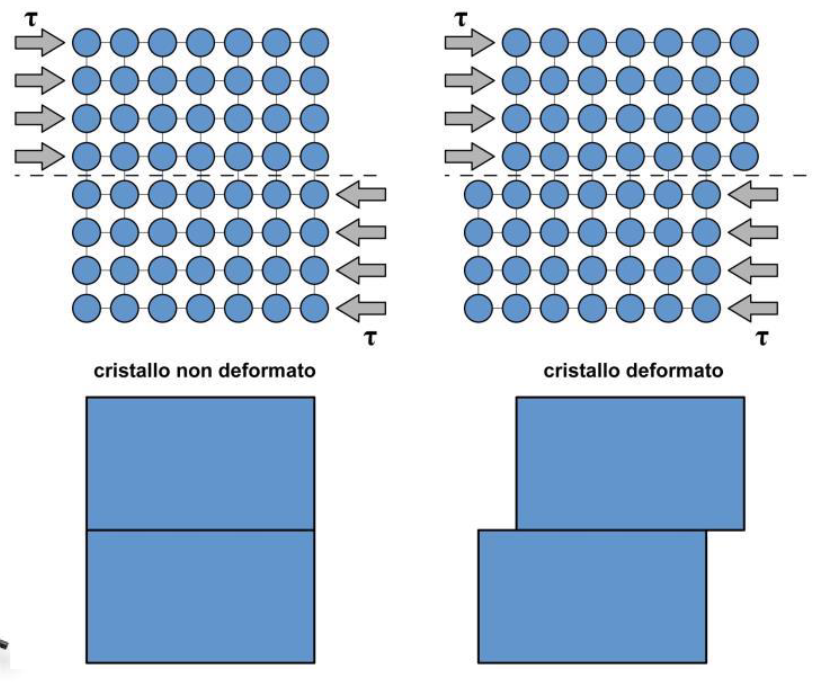
\includegraphics[width=.85\linewidth]{Deformazione di Dislocazione.png}
                \end{figure}
                Per muovere le dislocazione occorre usare la sforzo/sollecitazione di taglio/scorrimento. Lo sforzo di taglio sottosposto viene simboleggiato dal simbolo $\tau$. La scorrimento cuase una rottura di tutti i legami e nello stesso istante la creazione di legami nuovi. \\
                \begin{figure}[h!]
                    \centering
                    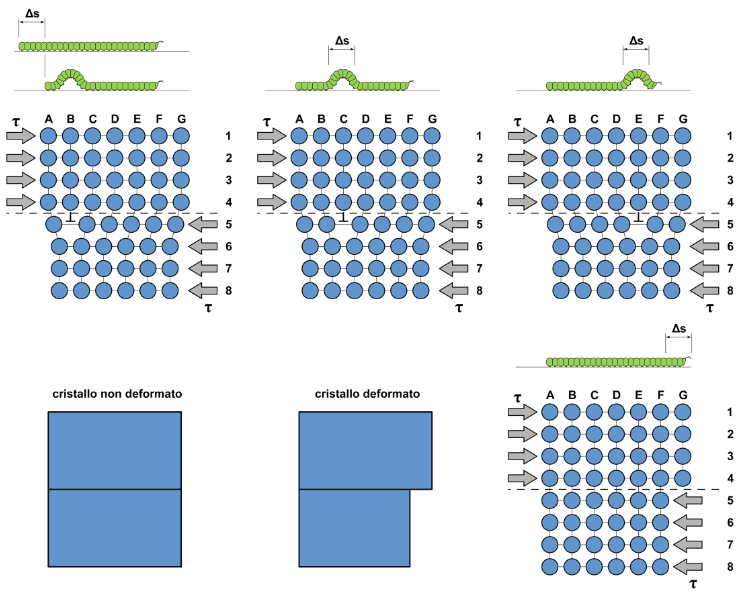
\includegraphics[width=.85\linewidth]{Scorrimento di Dislocazione.png}
                \end{figure}
                Con sforzi le deformazioni possono muovore le dislocazioni, quando la dislocazione \'e spostata fino alla fine del cristallo il cristallo diventa deformato se stesso. Rimuovendo le dislocazioni solo le parti adiacenti alla dislocazione si muovono per rimuovere la dislocazione, per ci\'o \'e considerato un'avanzamento progressivo di salti reticolari.\\ \\
                Praticamente deformare un reticolo con dislicazioni costo molto meno energeticamente (di fattori molto alti), e permette la deformazione del reticolo.\\
                90\% del moto reticoloare \'e a cause delle dislocazioni.\\ \\
                In generale, pi\'u dislocazioni sono presenti nel materiale pi\'u \'e maleabile, e le deformazioni pi\'u sono permesse di viaggiare pi\'u \'e deformabile il materiale per ci\'o meno resistente. Per sommare, le dislocazioni agevolano la deformazione.\\ \\
                Le dislocazioni permettono di ridurre la energia che serve per le deformazioni, la diminuizione nella energia \'e di fattori molto grandi.
        \subsection{Altri Rafforzamenti di Materiale}
            Come visto nel rafforzamento per alligazione (rafforzamento per soluzione solida), i rafforzamenti sono metodi per rendere il materiale pi\'u resistente attraverso diversi processi.
            \subsubsection{Rafforzamento per incrudimento}
                \begin{figure}
                    \centering
                    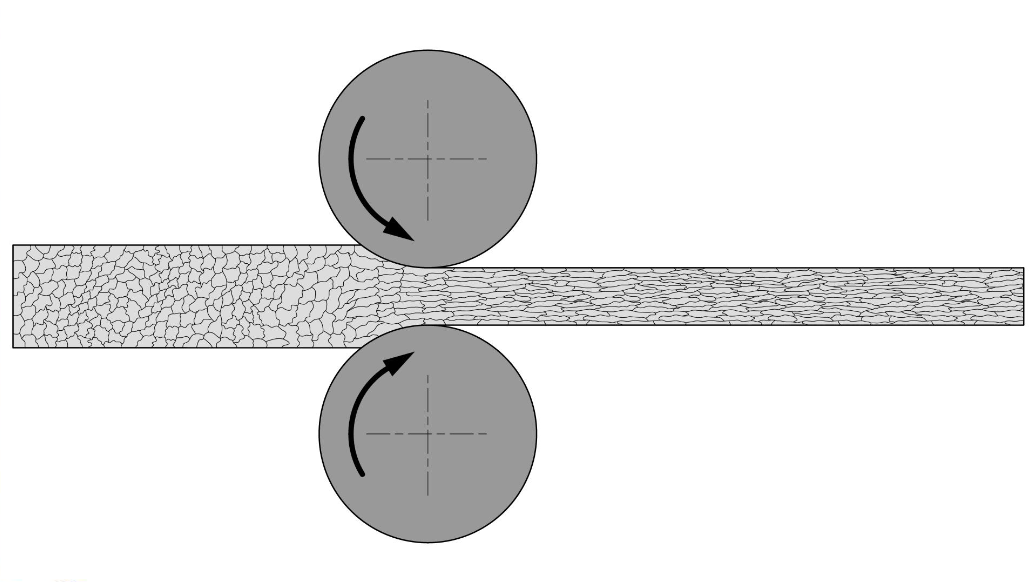
\includegraphics[width=.80\linewidth]{Rafforzamento per Incrudimento.png}
                \end{figure}
                Il rafforzamento per incrudimento \'e in base, schiacciare il metallo o lega mentre \'e freddo, detto deformazione a freddo. Durante la deformazione si allungano i grani nella direzione perpendicolare alle forze applicate.\\ \\
                La deformazione a freddo mette in moto le dislocazioni, pi\'u si deforma il materiale pi\'u energia ci vuole perch\'e le dislocazioni a bassa energia sono esaurite e rimangono le dislocazioni ad altra energia.\\
                Quando si deforma a freddo (incrudire) si aumenta la resistenza perch\'e si rimuovono le dislocazioni a bassa energia, quindi \'e pi\'u difficile muovere le dislocazioni rimaste. Pi\'u si deforma, pi\'u \'e resistente.\\ \newpage
                \begin{figure}[ht]
                    \centering
                    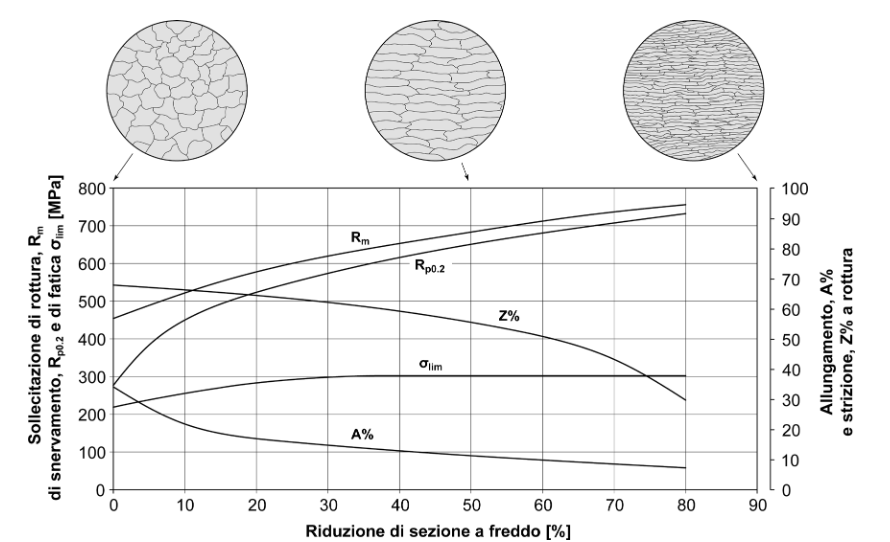
\includegraphics[width=\linewidth]{Grafico di Cambio Sezione.png}
                \end{figure}
                Quando si deforma a freddo aumentano le dislocazioni, per\'o si bloccano l'un l'altro rendendo la struttura pi\'u resistente. L'effetto di aumento di dislocazioni \'e noto come moltiplicazioni di dislocazioni e causa il rinforzamento di del reticolo.\\
                L'aumento di dislocazioni significa che il muoviment si blocchi.
                \begin{figure}[!h]
                    \centering
                    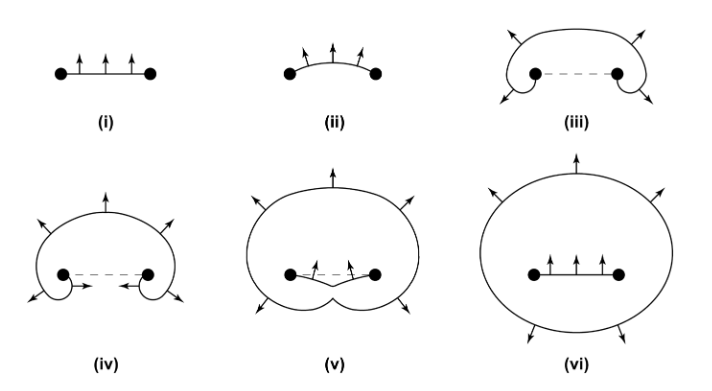
\includegraphics[width=.85\linewidth]{Grafico per Meccanismo Frank-Read.png}
                    \caption{Meccanismo Frank-Read}
                \end{figure}
                Il meccanismo Frank-Read rappresenta la interazione tra due ostacoli e una dislocazione che \'e a questi due ostacoli. La linea rappresenta la linea della dislocazione e le freccie la direziione del moto della dislocazione. Gli anelli generati continuano a diventare pi\'u grandi e non rimangono statici, mentre la dislocazione originale continua a generare pi\'u dislocazioni nuove. Quest'effetto \'e la ragione per l'aumento nel numero delle dislocazioni.
            \subsubsection{Rafforzamento per precipitazione}
                In questo caso la precipitazione viene intesa come mettere altri materiali, composti o metalli, nel materiale originale per rinforzare il materiale.
                \begin{figure}
                    \centering
                    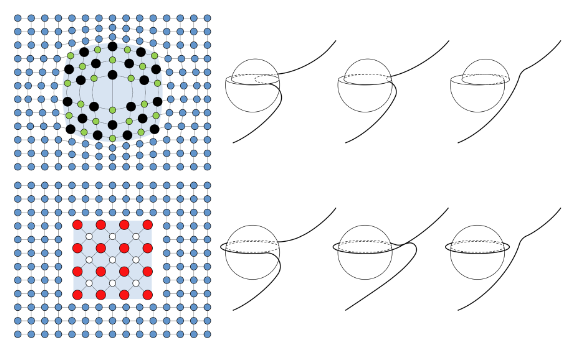
\includegraphics{Composti coerenti e incoerenti e la loro interazione con le dislocazioni.png}
                \end{figure}
                I materiali agiscono come ostacoli per le dislocazioni a cui si possono ancorare, come visto nel esempio di Frank-Read, ma anche some ostacoli temporanei che causano temporaneamento solo il rallentamento del moto della .\\
                Durante il moto delle dislocazioni i precipitati (composti o altri metalli) sono ostacoli per le dislocazioni. I composti incoerenti rallentano il moto della dislocazione, causando la creazione di un altra dislocazione.\\
                I composti coerenti in vece, a causa della loro equa direzione in confronto al reticolo inglobante vengono tagliati e spostati a causa della interazione con le dislocazioni. A causa del requisiti di rottura di legami (cio\'e viene richiesta pi\'u energia) i composti coerenti occoro essere un ostacolo pi\'u grande per le dislocazioni, per\'o non causano la creazione di nuove dislocazioni.\\
                \begin{figure}
                    \centering
                    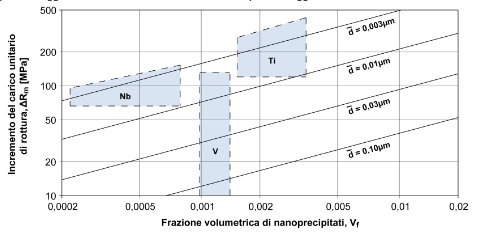
\includegraphics{Diagramma collerazione tra finitura di matlli e l'aumento in resistenza nel materiale.png}
                \end{figure}
                Questo diagramma fa vedere che i precipitati di diametro p\'u piccolo hanno un effetto pi\'u grande sulla durezza rispetto alla looro frazione volumentrica in confronto ai precipitati pi\'u grandi.\\
                La alligazione causa la reazione di metalli e atomi interstiziali come C e N per creare composti nella legha (alcuni esempi sono il vanadio (V) che forma VC, il niobio(Nb) che forma NbC e Nb(CN), o il titanio (Ti) che forma TiC). Questi allegazioni sono classificate come High Strength Low Alloyed (HSLA), a causa del loro effetto grande sulla resistenza del materiale anche a bassi percentuali volumetriche (~.2\%). A causa della bassi percentuali volumetriche possono esser chiamate anche micro-allegazioni, cio\'e aggiungere metalli per creare composti per aumentare le dislocazioni.\\ \\
                \underline{\textbf{IMPORTANTE:}} Si possono usare tutte e tre i metodi di rafforzamento per aumentare la resistenza.\\ 
                Per\'o in generale per il rafforzamento per precipitazione pi\'u fini sono i precipitati pi\'u incrementa la resistenza. Cio\'e per aumentare la resistenza servono pi\'u precipitanti pi\'u piccoli.\\
        \subsection{Difetti di superfice : bordi grano}
            I metalli si solidificano in gruppi, per\'o non si incontrano bene e creano grani. \\ \\
            Dopo aver sciolto un metallo, pi\'u si abbassa la temperatura, statisticamente in alcuni punti si formano dei grani (nuclei iniziali della solidificazione), a forma CCC,CFC o HCP (o altre che a cui non abbiamo guardato). A causa della creazione dei grani, gli atomi iniziano ad attaccarsi, nella stessa forma reticolare, come mattoni in un muro che seguono uno stesso modello ricorrente. Questo processo si chiama nucleazione e accrescimento.\\ \\
            Si formano edifici cristallografici (\underline{nome giust}), pero visto che sono cresciuti indipendentemente, al confine la struttura non \'e come nessuno dei due edifici perch\'e la struttura sta provando a far parte di tutti e due gli edifici quindi crea un reticolo che non \'e a nessuno dei due. A causa della struttua disorganizzata ci stanno meno atomi in questa zona, come una fossa fra due campi.
            \begin{figure}
                \centering
                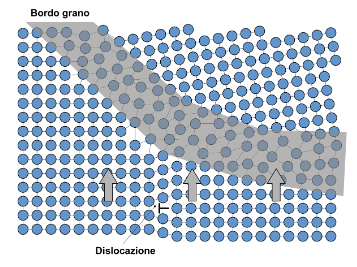
\includegraphics{Diagramma bordo grano.png}
                \caption{La zona di borda, che \'e meno densa e colorata in grigio.}
            \end{figure}
            La dislocazione si muove dentro al grano per\'o si ferma al bordo grano perch\'e non ha un reticolo uguale. Questo blocco delle dislocazione \'e la causa del rafforzamento del reticolo, e la ragione perch\'e pi\'u dislocazioni \'e meglio.
        \subsection{Rafforzamento per affinimento del grano}
            \begin{figure}
                \centering
                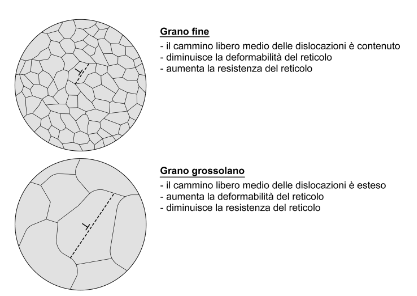
\includegraphics{Differenza dimensioni grnao.png}
            \end{figure}
            I grani pi\'u fini sono migliori perch\'e le dislocazioni non possono viaggiare molto, rendendo il materiale meno deformabile, e incontrano i bordi grano pi\'u velocemente rendondo il reticolo pi\'u resistente. I bordi grano sono buoni perch\'e bloccano le dislocazioni e per ci\'o aumentando la resistenza del reticolo.
        \subsection{Sintesi di Meccanismi di Rafforzamento}
            \begin{itemize}
                \item Rafforzamento per soluzione solida (alligazione)
                \item Rafforzamento per incrudimento
                \item Rafforzamento per precipitazione
                \item Rafforzamento per affinimento del grano
            \end{itemize}
        \subsection{Diffetti di Volume - I diffetti che non vogliamo}
            \subsubsection{Cavit\'a}
                La cavit\'a (anche fori) sono discontinuit\'a volumetriche che rendono il materiale meno resistente agli sforzi.\\ \\
                \underline{\textbf{Cause:}} \\
                \underline{Porosit\'a da gas}, pu\'o capitare se il materiale \'e colate e viene intrappolato del gas, causando un cavit\'a.\\
                \underline{Cavit\'a di ritiro}, quando il metallo \'e colato negli e si solidifice a causa il volume si diminuisce e causa ritiri. Questi occorro di solito ai bordi del grano perch\'e sono le ultime a solidicarsi.
            \subsubsection{Cricche}
                Una cricca \'e una frattura microscopica, questo \'e pi\'u critico perch\'e \'e pi\'u appuntito, e in generale le deformazioni a bordi appuntito sono peggiori delle deformazioni a bordi arrotondato come le cavit\'a.
            \subsubsection{Inclusioni}
                Il volume dei materiali che sono occupati da materiali diversi che sono completamente inglobati. \\ \\
            In generale nei diffetti \'e pi\'u importante la forma che le dimensioni.
    \section{Lezione 5 - Diffusione e Prove Meccaniche}
        \subsection{Diffusione}
            La diffusione \'e il modo in cui gli atomi si muovono allo stato solido dentro al reticolo. Si muovono pi\'u velocamente pi\'u \'e alta la temperatura. Cio\'e pi\'u \'e alta la temperatura pi\'u \'e alta la mobilit\'a degli atomi.
            \subsubsection{Autodiffusione (per vacanze)}
                Usando le vacanze gli atomi si ponossono muovere. Se non ci fosser le vacanze gli atomi non si muoverebbero.
                \begin{figure}[!h]
                    \centering
                    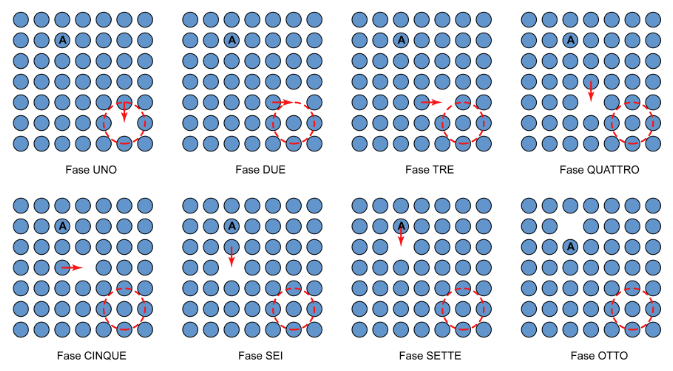
\includegraphics[width=.85\linewidth]{Autodiffusione per vacanze.png}
                \end{figure}
            \subsubsection{Interdiffusione in sistemi eterogenei (per vacanze)}
                La interdiffusione in sistemi eterogeni occorre per effetto delle presenza di vacanze. Due solidi eterogenei, con atomi di dimensione simile,scambiano atomi fra loro e con tempo diventano omogenei.\\ \\
                La concentrazione degli atomi nei due spaci cambia con tempo e spazio.
                \begin{figure}[!h]
                    \centering
                    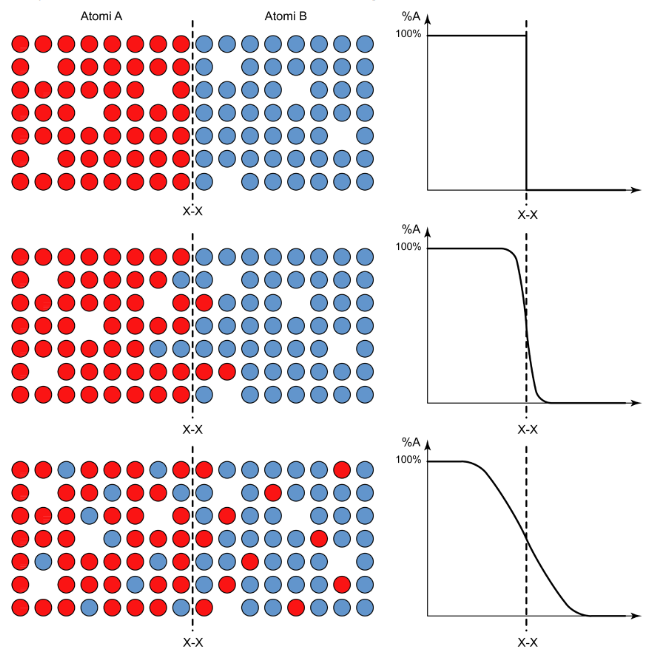
\includegraphics[width=.75\linewidth]{Interdiffusione in sistemi eterogeni (per vacanze).png}
                \end{figure}
            \subsubsection{Interdiffusione in sistemi per eterogenei (per lacune)}
                Nella interdiffusione in sistemi eterogenei occorre quando dei gas permeano il metallo, sfruttando le lacune per diffondere atomi, specialmente per atomi interstiziali.\\ \\
                Bisogna ricordarsi che la lacune sono gli spazi vuoti fra gli atomi. E come ultima nota, questo processo succede ad alta T nell'accaio.
                \begin{figure}[!h]
                    \centering
                    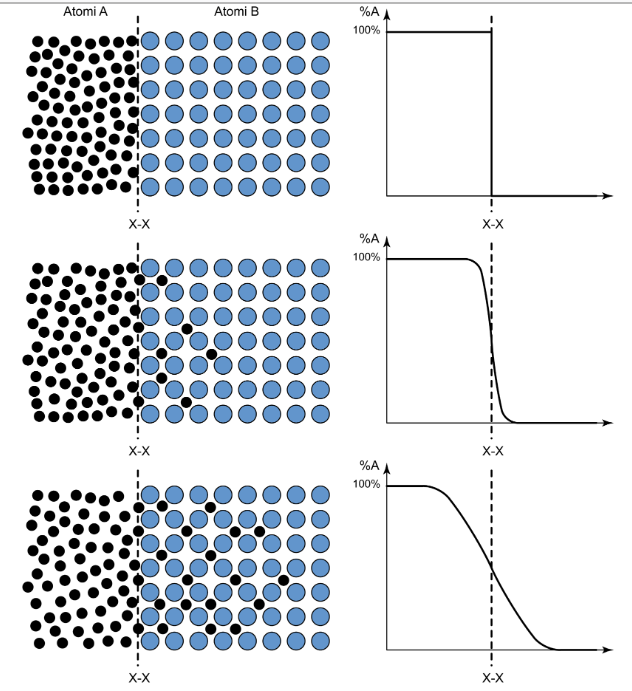
\includegraphics[width=.75\linewidth]{Interdiffusione in sistemi eterogeni (per lacune).png}
                \end{figure}
        \newpage
        \subsection{Prove meccaniche dei materiali metallici}
            Le prove meccaniche sono prova a cui materiali sono posti per trovare i loro limiti di deformazione e sforzo
            \subsubsection{Definizione di sforzo ($\sigma$)}
                Lo sforzo, o sollecitazione, \'e una unit\'a di misura della forza applicata per unit\'a di area quadra.
                \begin{figure}[!h]
                    \centering
                    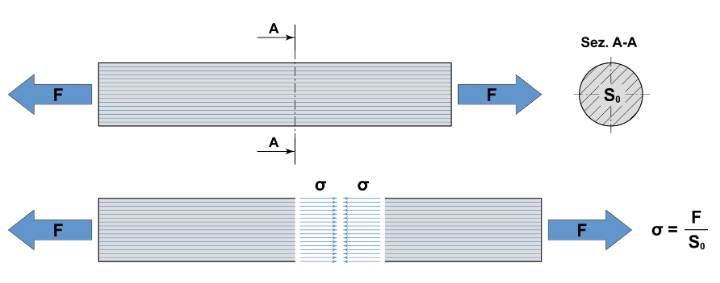
\includegraphics[width=.85\linewidth]{Diagramma definizione dello sforzo.png}
                \end{figure}
                Il diagramma rappresenta la definizione dello sforzo, le freccie piccole sono gli sforzi che sono applicati al materiale su area di mm$^2$, questi sforzi, mulitiplicato per l'area su cui viene applicato, arriva alla forza totale. \'E importante distinguere lo sforzo dalla forza, lo sforzo \'e la forza applicata su un area di 1mm$^2$ o si pu\'o dire che \'e il rapporta tra la forza e l'area su cui ha effetto.\\
                La sforzo ha il simbolo $\sigma$(sigma) e le sue unita sono $\frac{N}{mm^2}$ o $MegaPascal (MPa)$.\\
                La analisi dimensionale \'e:
                \begin{equation*}
                    \sigma = \frac{F}{S_o} = \frac{[N]}{[mm^2]} \equiv MPa
                \end{equation*}
            \subsubsection{Definizione di deformazione ($\epsilon$)}
                La deformazione \'e una unit\'a di misura, della percentuale di allungamento di un materiale quando questo materiale \'e sottoposto a forze.\\
                \begin{figure}
                    \centering
                    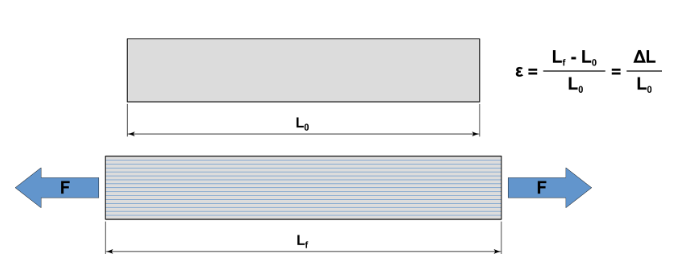
\includegraphics{Diagramma definizione della deformazione.png}
                \end{figure}
                La deformazione \'e il l'allungamento (cambio di lunghezza) di un materiale rispetto alla lunghezza originale ed \'e adimensione perch\'e \'e una lunghezza diviso una lunghezza.
                Un allengamento($\Delta L$) di un sistema occorre nella direzione della forza applicata. Sia la forza e l'allungamento dipendenon dalle dimensioni dei componenti, mentre lo sforzo e la deformazione sono propriet\'a del materiale, e non dipendono da niente.
            \subsubsection{Esempi}
                Gli esempi sono nel quaderno, per\'o spiego la roba importante.\\ \\
                Per avere lo stesso effetto su in materiale bisogna considerare l'area, perch\'e pi\'u pi\'u forza bisogna applicare. Invece lo sforzo \'e invariante all'area. Per ci\'o se si pensa in metodo unitario \'e meglio considerare lo sforzo che la forza, perch\'e lo sforzo \'e una propreit\'a fisica.\\ \\
                in funzione della lunghezza iniziale, la deformzaione cambia. In funzione della sezione lo sforzo cambia. Per ci\'o bisogna pensare in termini di $\frac{F}{A}$ non F, perch\'e f dipende dall'area mentre la sforzo \'e intriseco del materiale e funzione dell'area.
        \subsection{Prova di trazione}
            Lo scopo della prova di trazione \'e di valutare la resistenza a una sollectiazione monoassiale di un provino di un materiale.\\ \\
            Viene sottposto un provino (di solito cilindrico) a un serie di forze progressivamente pi\'u grandi.\\ \\
            Misurando le forza applicata su e l'allungamento del provino, si possono derivare lo sforzo e la deformazione di un provino di un raggio specifico.
            \begin{figure}[ht!]
                \centering
                \begin{subfigure}{.45\linewidth}
                    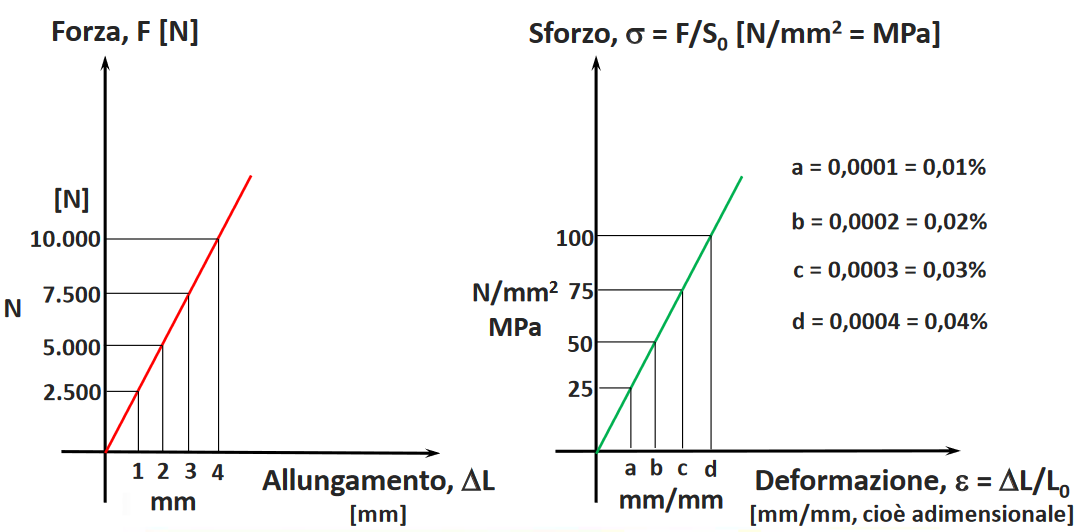
\includegraphics[width=\linewidth]{Diagramma prova di trazione 1.png}
                \end{subfigure}
                \begin{subfigure}{.45\linewidth}
                    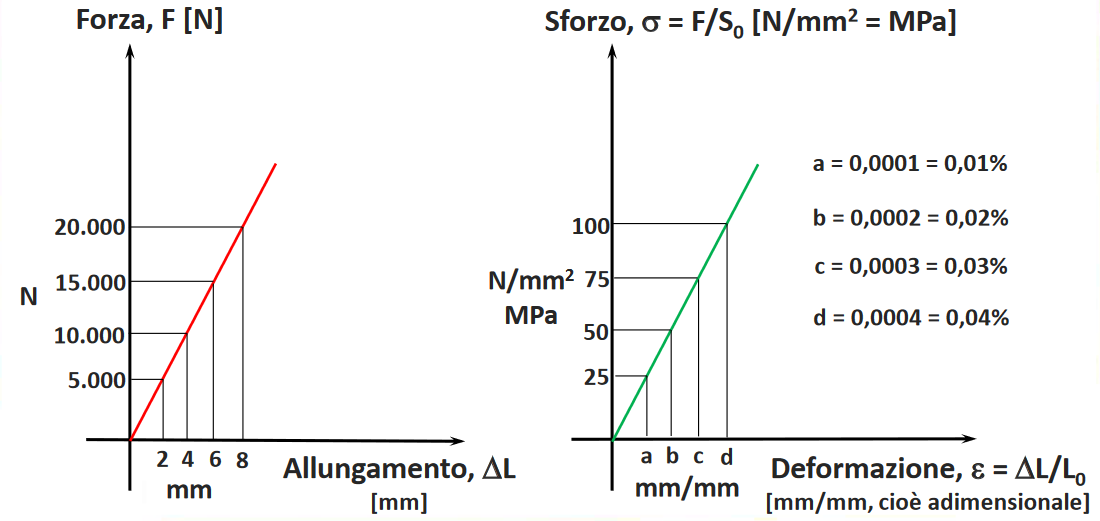
\includegraphics[width=\linewidth]{Diagramma prova di trazione 2.png}
                \end{subfigure}
            \end{figure}
            Nella immagine alla destra il diametro e lunghezza del pezzo \'e aumentata di un fattore di due, e in corrispondenza la forza \'e aumentata (anche l'allungamento) dello stesso fattore, per\'o lo sforzo e la deformazione sono rimasti uguali, questo fa vedere che lo questi due sono propriet\'a fisiche del materiale quindi rimangono uguali indipendenti della forza o della sezione.
        \subsection{Tipi di Provino}
            Ci sono alcuni tipi di provino, per\'o sono tutti normalizzati.
            \begin{figure}[!h]
                \centering
                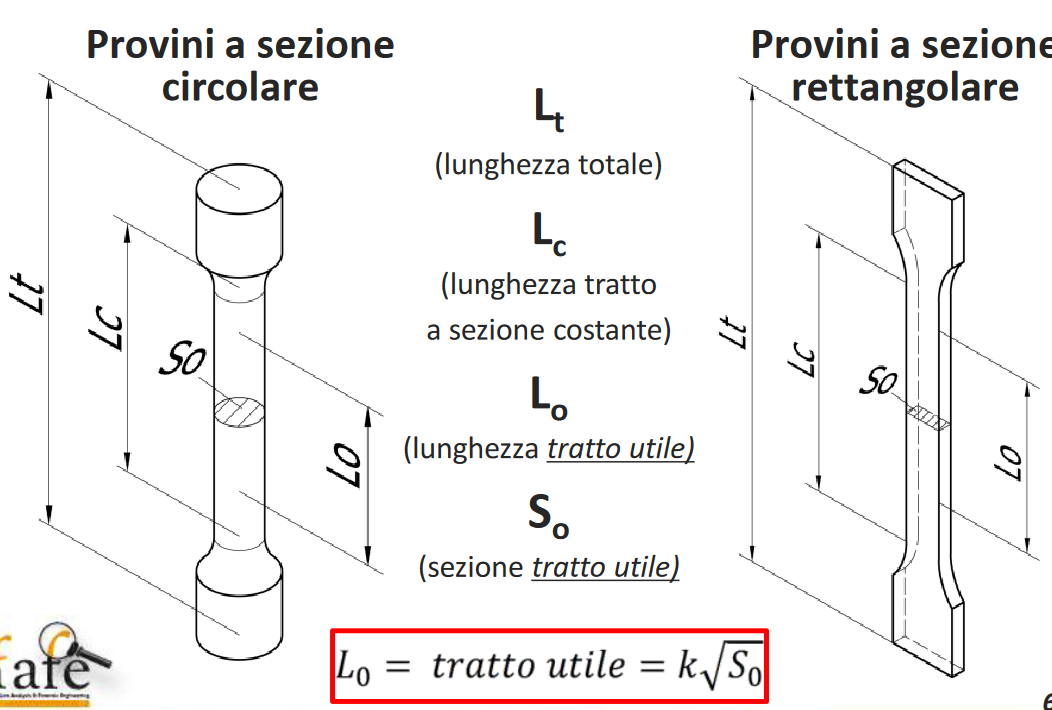
\includegraphics[width=.85\linewidth]{Diagramma tipi di provino.png}
                \caption{Il valore k = 5,56}
                \label{fig:my_label}
            \end{figure}
        \newpage
        \subsection{Macchina di Prova}
            \begin{figure}[h!]
                \centering
                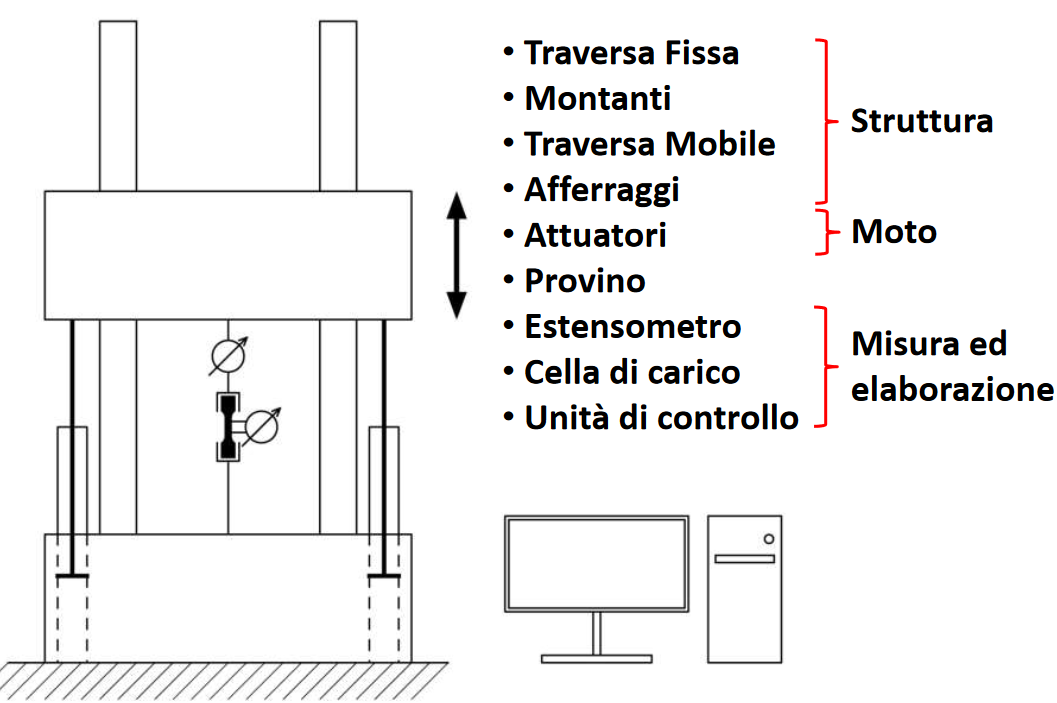
\includegraphics[width=.85\linewidth]{Diagramma macchina di prova.png}
            \end{figure}
            Le macchine di prova vengono usate per misurare lo sforzo e la deformazione di un provino. La cella di carico, in simbolo sopra il provino, misura la forza che viene applicata, mentre il estensometro misura l'allugamento del materiale, per poi esser mandato al computer per fare i calcoli.
        \subsection{Tipi di Curve Risultanti}
            \begin{figure}[!h]
                \centering
                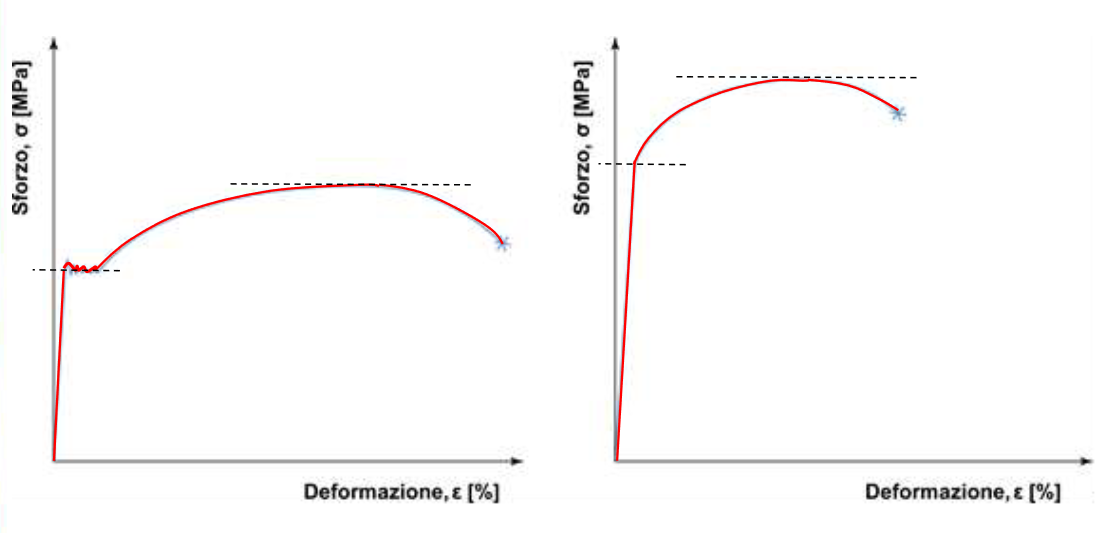
\includegraphics[width=.85\linewidth]{Tipi di Curve da Prova di Trazione.png}
            \end{figure}
            Questo sono due tipi di diagrammi che si possono ricevere dalla prova di trazione. Questo che si pu\'o notare \'e che tutte e due le curve iniziano lineari e a certo punto iniziano a curvare, questo punto \'e il punto dove la deformazione va da essere elastica a plastica.\\
            Le assi non sono dimensionata, ma si pu\'o comprendere che pi\'u un materiale \'e deformabile meno sforzo c\'e bisogno, e meno deformabile pi\'u sforzo c'\'e bisogno (a causa del moto delle dislocazioni). 
            \begin{figure}[h!]
                \centering
                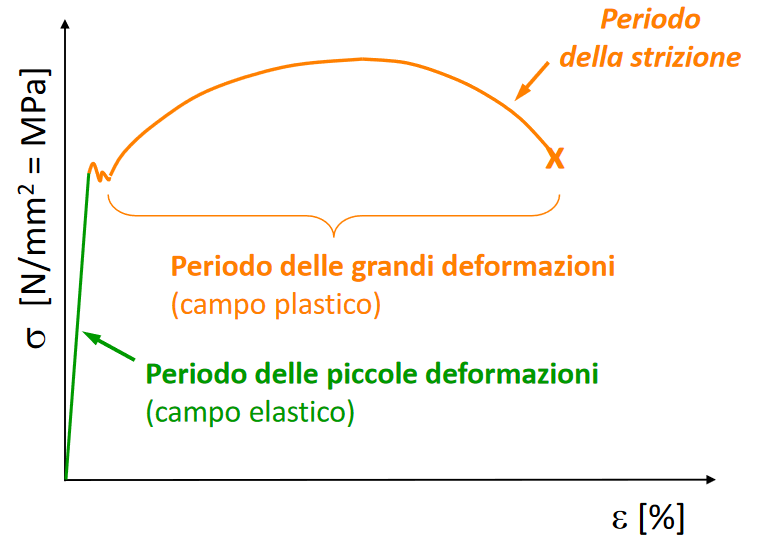
\includegraphics[width=.85\linewidth]{Diagramma sezionato di curva da prova di trazione.png}
            \end{figure}
        \subsection{Campo elastico}
            Nel campo elastico il materiale si deforma sotto forzema dopo ritorna alla forma originale. Il Modulo Eastico Longitudinale(E), o,Modulo Young, \'e il coefficiente angola nella relazione tra sforzo e deformazioni, cio\'e quanto sforzo produce una certa deformazione. Il Modulo Elastico \'e un parametro fisico, non meccanico, perch\'e a causato dalle interazioni attrattive elettromagnetiche nei materiali.\\ \\
            {\textbf{\'E importante sapere che ogni materiale, metallico, ceramico o polimerico ha un module elastico perch\'e tutti possono esser sottoposti a deformazioni elastiche.} Quando si raggiunge il campo plastico, non \'e pi\'u possibile ritornare al campo elastico.
            \begin{figure}[!h]
                \centering
                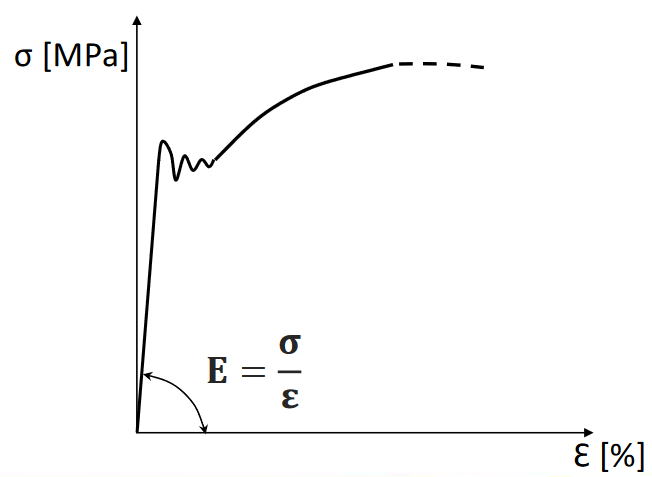
\includegraphics[width=.85\linewidth]{Diagramma per il modulo di elasticita.png}
            \end{figure}        
    \section{Lezione 6 - Continuazione della Ultima Lezione}
        Nell'campo elastico $\sigma = E \dot \epsilon$
        Le dislocazioni non cci stano ancore muovendo.
        \subsection{Continuazione di Prova di Trazione}
            \subsubsection{Termine Campo Elastico}
                A un certo livello di sforzo le dislocaizoni iniziano a muoversi e le deformaioni snon sia elastiche che plastiche. Sono anche elastiche perch\'e la formazioni elastiche non se ne vanno mai via.
            \subsubsection{Carico unitario di Snervamento (R$_sn$ o $\sigma_sn$)}
                Il carico unitario di snervamento \'e il punto dove le dislocazioni iniziano a muoversi, e definisce lo spostamento di grandi deformazioni invece piccole deformazioni.\\ \\
                \begin{figure}[!h]
                    \centering
                    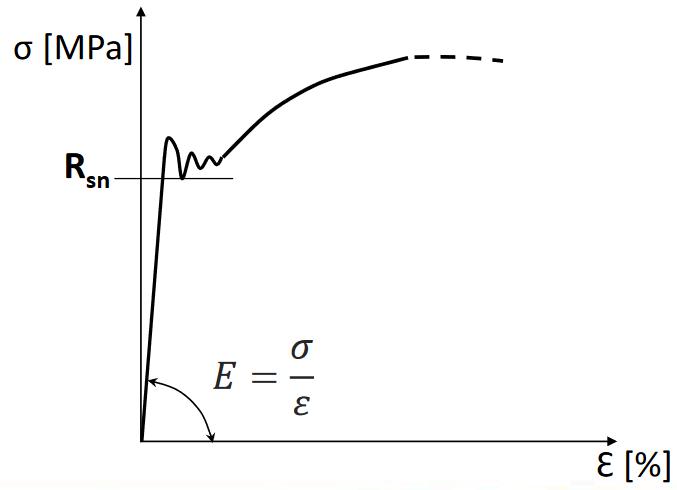
\includegraphics[width=.85\linewidth]{Carico Unitario di Snervamento.png}
                \end{figure}
                A questi sforzi il comportamento del materiale inizia a cambiare e la estensione non \'e pi\'u lineare in confronto allo sforzo.
            \subsubsection{Carico unitario di snervamento (R$_p 0,2$)}
                \begin{figure}[!h]
                    \centering
                    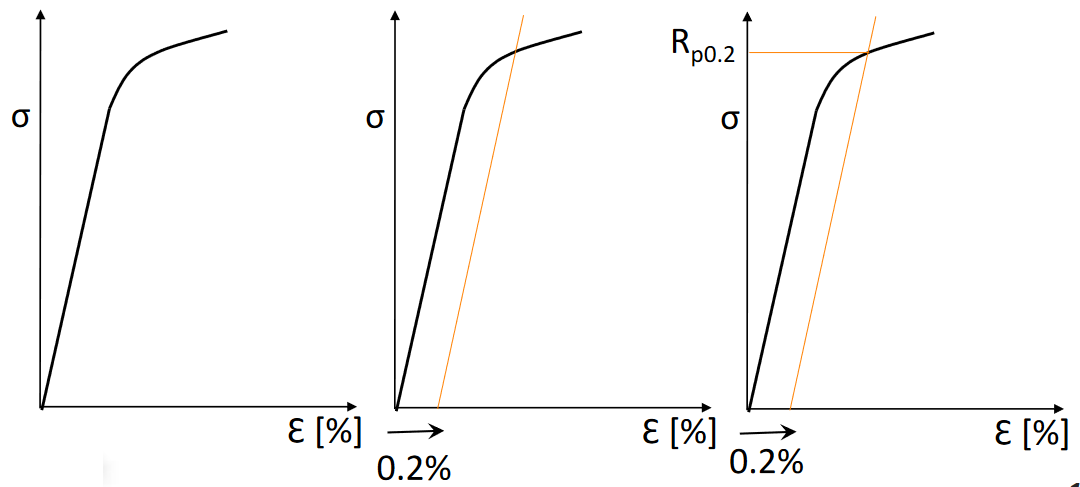
\includegraphics[width=.85\linewidth]{Carica Unitario di Snervamento p02.png}
                \end{figure}
                Invece di definire R$_sn$, si definisce il carico dalla prpporzionalit\'a lineare dello $0,2\%$\\ \\
                R$_p 0,2$ rappresentano la stessa cosa di R$_sn$ quando non \'e evidente il punto di cambio da elastico a plastico. Si prende il tratto lineare iniziale e si traccia una retta parallela che inizia al $0,2\%$. Cio\'e $\epsilon = 0,2\% o \epsilon = 0,002$.\\ \\
                Se il grafico ha una discontinuit\'a R$_sn$ e se c'\'e una continuit\'a R$_p 0,2$, hanno lo stesso obbiettivo.\\ \\
                Quando R$_sn$ o R$_p 0,2$ sono superate si entra nel campo plastico dove la deformazioni diventano permanenti oltre le deformazioni plastiche e le deformazioni vanno da essere piccole a grandi.\\ \\
                Il componente quando il carico \'e tolto, ritorno alla base seguendo E, e arriva a una nuova lunghezza, che \'e la nuova forma, cio\'e permanente.
            \subsubsection{Carico Massimo (R$_m$)}
                 \begin{figure}[!h]
                    \centering
                    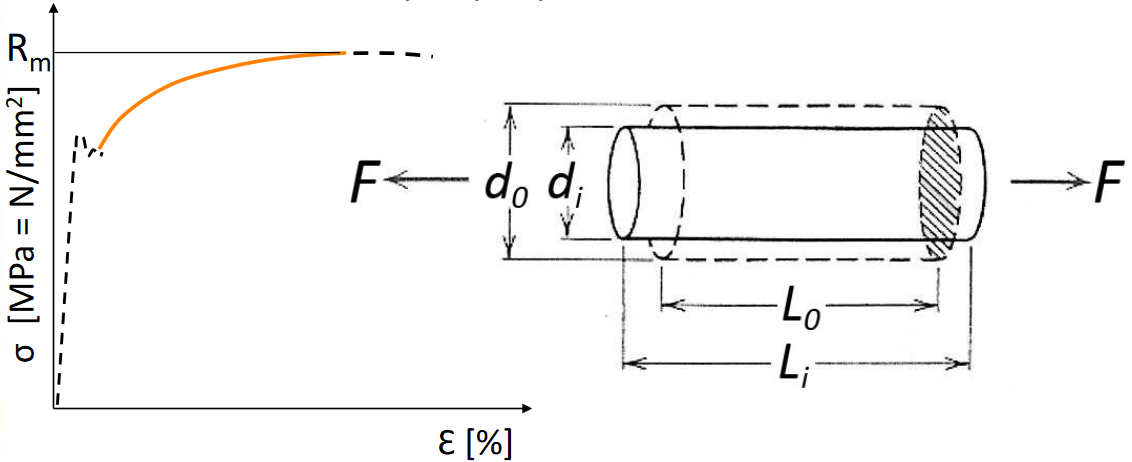
\includegraphics[width=.85\linewidth]{Carico Unitario Massimo.png}
                \end{figure}
                 R$_m$ \'e lo sforzo massimo. \'E noto come il carico massimo o il carico di rottura, anche se a questo punto non c'\'e rottura. Pi\'u alto \'e R$_m$ pi\'u resistente \'e il materiale.
                 Tra R$_sn$ e R$_m$, la deformazione \'e uniforme. Pi\'u sforzo, pi\'u diminuisce la sezione. la sezione si ristringe uniformemente. R$_m$ \'e il pi\'u importante perch\'e \'e il carico massimo.
            \subsubsection{Dopo il carico massimo}
                \begin{figure}[!h]
                    \centering
                    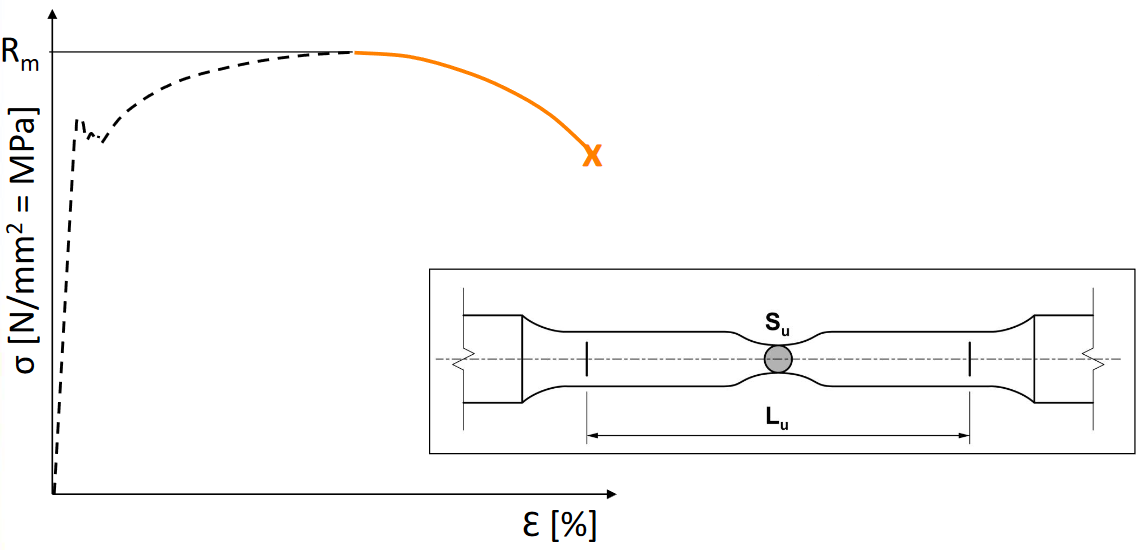
\includegraphics[width=.85\linewidth]{Campo di Strizione.png}
                \end{figure}
                Dopo R$_m$, la deformazione inizia a concentrarsi in un punto, a effetto della strizione. Lo sforzo diminuisce perch\'e si sta diminuendo la sezione, quindi ci vuole meno forza, per estendere il provino.\\ \\
                R$_m$ \'e il pi\'u importante perch\'e \'e il carico massimo.
                \begin{figure}[!h]
                    \centering
                    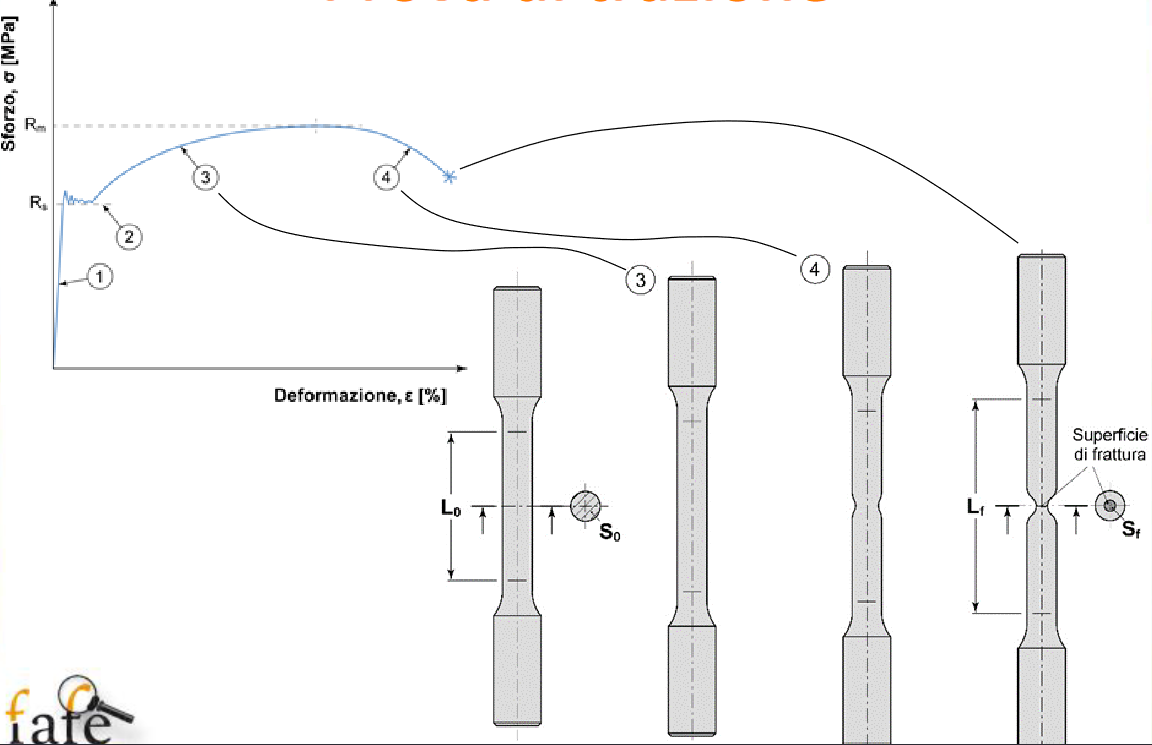
\includegraphics[width=.85\linewidth]{Prova di Trazione - Cambio in Sezione.png}
                \end{figure}
        \subsection{Altri Parametri}
            Dopo la rottura si misura la lunghezza totale e la sezione finale. L$_u$ \'e l'ultima lunghezza prima di rottura.
            \begin{figure}[!h]
                    \centering
                    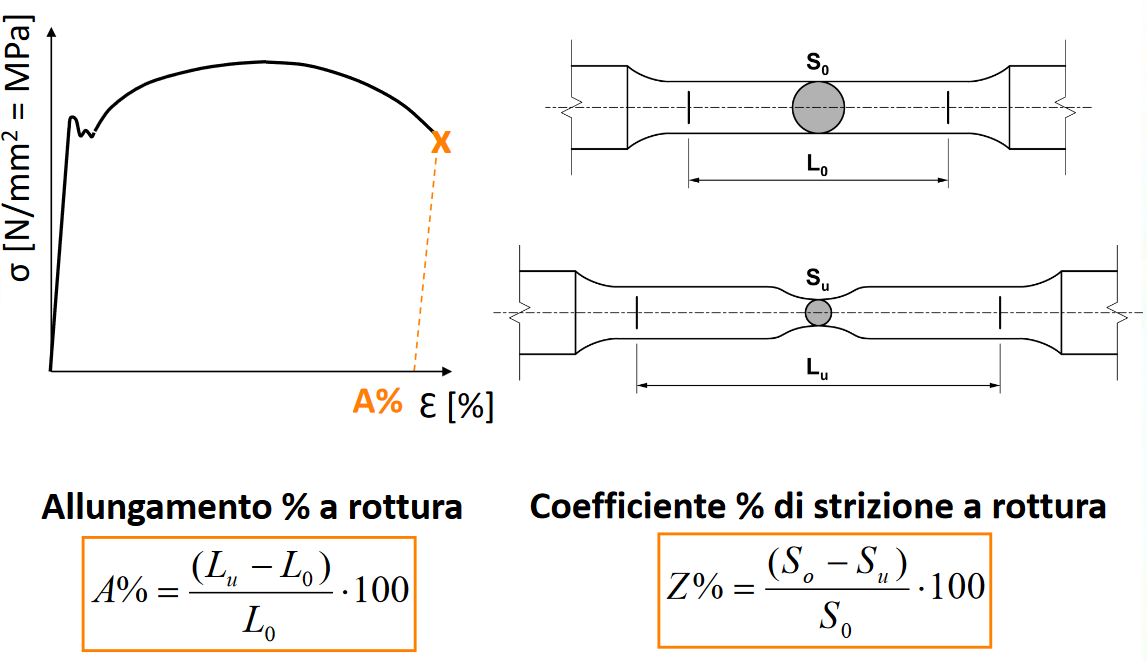
\includegraphics[width=.85\linewidth]{Grafico e Equazioni di Allungamento e Strizione a Rottura.png}
            \end{figure}
            L'allungamento a rottura \'e l'allungamento plastico del provino alla rottura. La strizione a rottura invece \'e una misura del cambio di sezione in confronto all'inizio. La formula generale \'e:
            \begin{equation*}
                \frac{\text{grande}-\text{piccolo}}{\text{iniziale}}
            \end{equation*}
            Invece se si interrompe la deformazione plastica, si pu\'o trovare l'allungamento effettivo facendo la somma della deformazione plastiche e la deformazione elastica. Perch\'e quando si rimuove lo sforzo la deformazione elastica ritorna a 0, mentre la deformazione plastica rimane.
        \subsection{Tipi di metalli}
            Un metallo pu\'o avere uno di due tipi di grafico, questi sono il grafico elastica lineare, che non ha un punto di cambio ben definito, e il grafico elasto-plastico, che ha un cambio ben definito. I materiali di tipo elastico lineare tendono ad essere fragili mentre quelli di tipo elasto-plastico tendono ad essere duttili.
            \begin{figure}[!h]
                    \centering
                    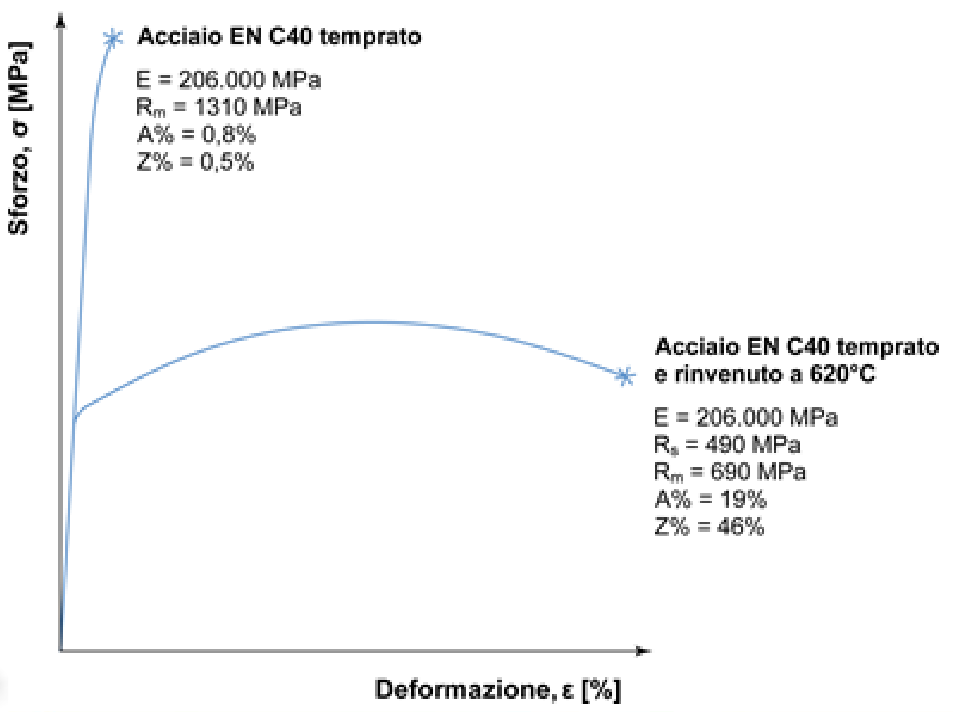
\includegraphics[width=.85\linewidth]{Esempio Elastico Lineare e Elasto-Plastico.png}
                    \caption{Alto-Elastico Lineare, Basso- Elasto-Plastico}
            \end{figure}
            Pi\'u carbonio, pi\'u resistente , ma meno deformabile. Cio\'e lo sforzo a cui le deformazioni occorrono aumentano, ma l'allungamento massimo diminuisce. Resistente significa quanto a sforzo pu\'o essere sottoposto un metallo. Per esempio all'aumentare dell'incruidmento la  resistenza aumenta, ma la deformazione diminuisce.
            \begin{figure}[!h]
                    \centering
                    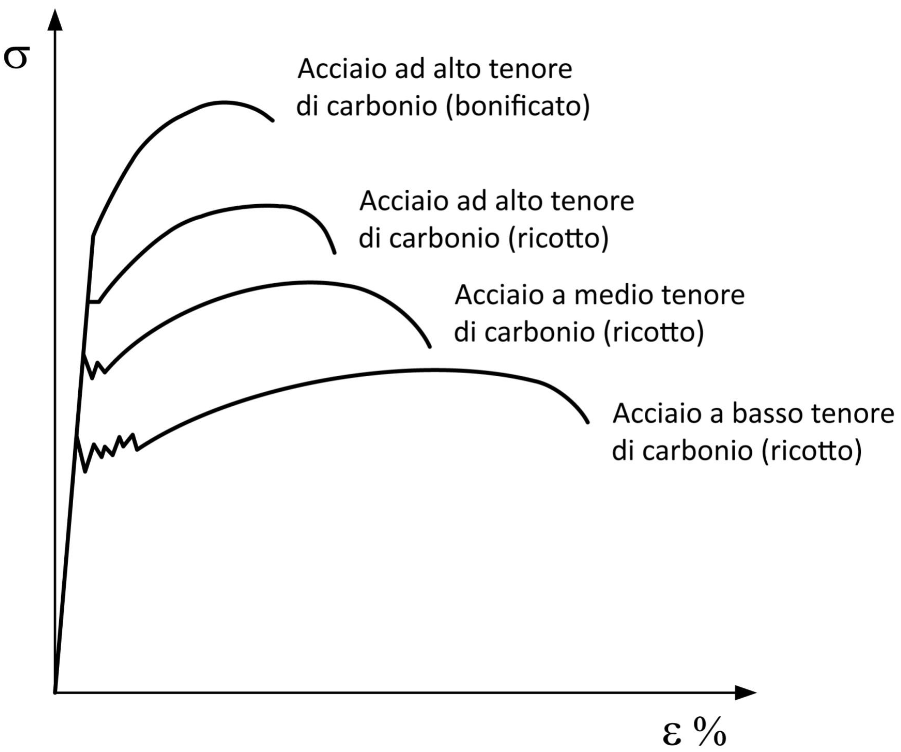
\includegraphics[width=.85\linewidth]{Grafici di Accaio con differenza di Carbonio.png}
            \end{figure}
            \begin{figure}[!h]
                    \centering
                    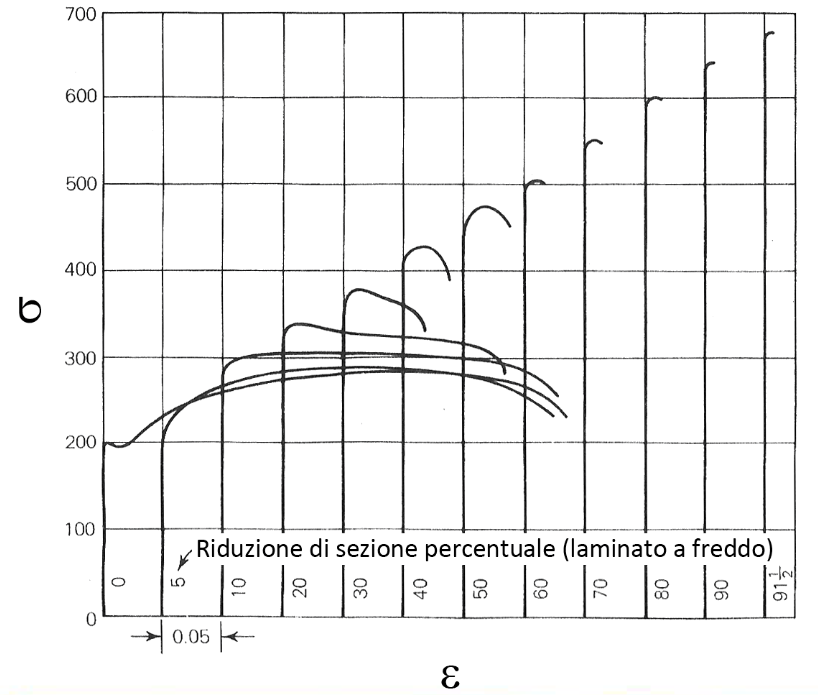
\includegraphics[width=.85\linewidth]{Grafico di Sforzo v. Allungamento con cambio di Incrudimento.png}
            \end{figure}
            \begin{figure}[!h]
                    \centering
                    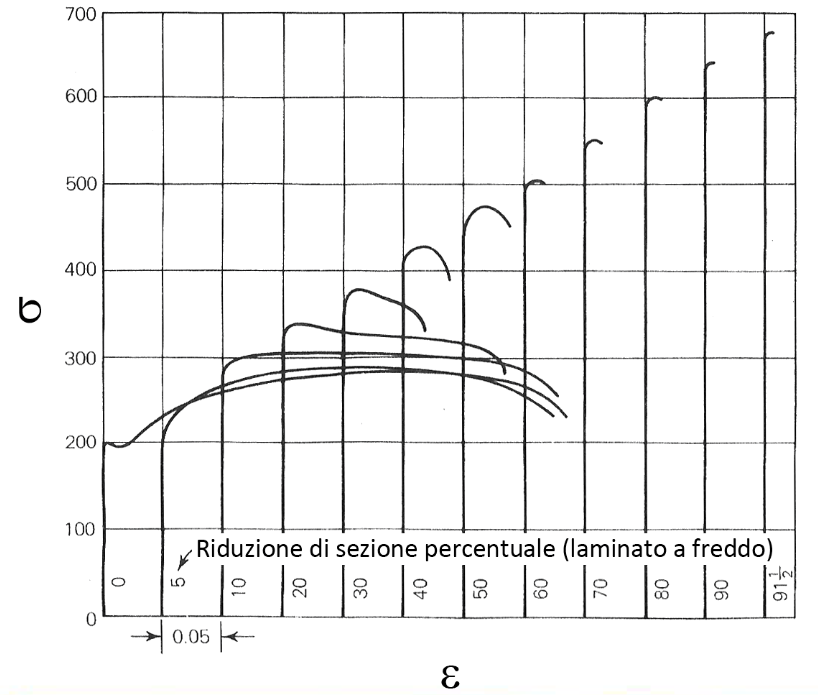
\includegraphics[width=.85\linewidth]{Grafico di Sforzo v. Allungamento con cambio di Incrudimento.png}
            \end{figure}
            Esempio di accaio vs. ghisa negli appunti
        \subsection{Lo scopo della prova di trazione e esempio di stato di sforzo}
            La prova di trazione trova il materiale nelle migliore condizioni specifiche del problema.\\ \\
            La stato di sforzo \'e lo sforzo a cui un materiale esemplare \'e sottoposto, invence il limite di resistenza ( di solito R$_sn$) \'e il limite di sforzo a cui un materiale pu\'o esser sicuramento sottoposto.
            \begin{figure}[!h]
                    \centering
                    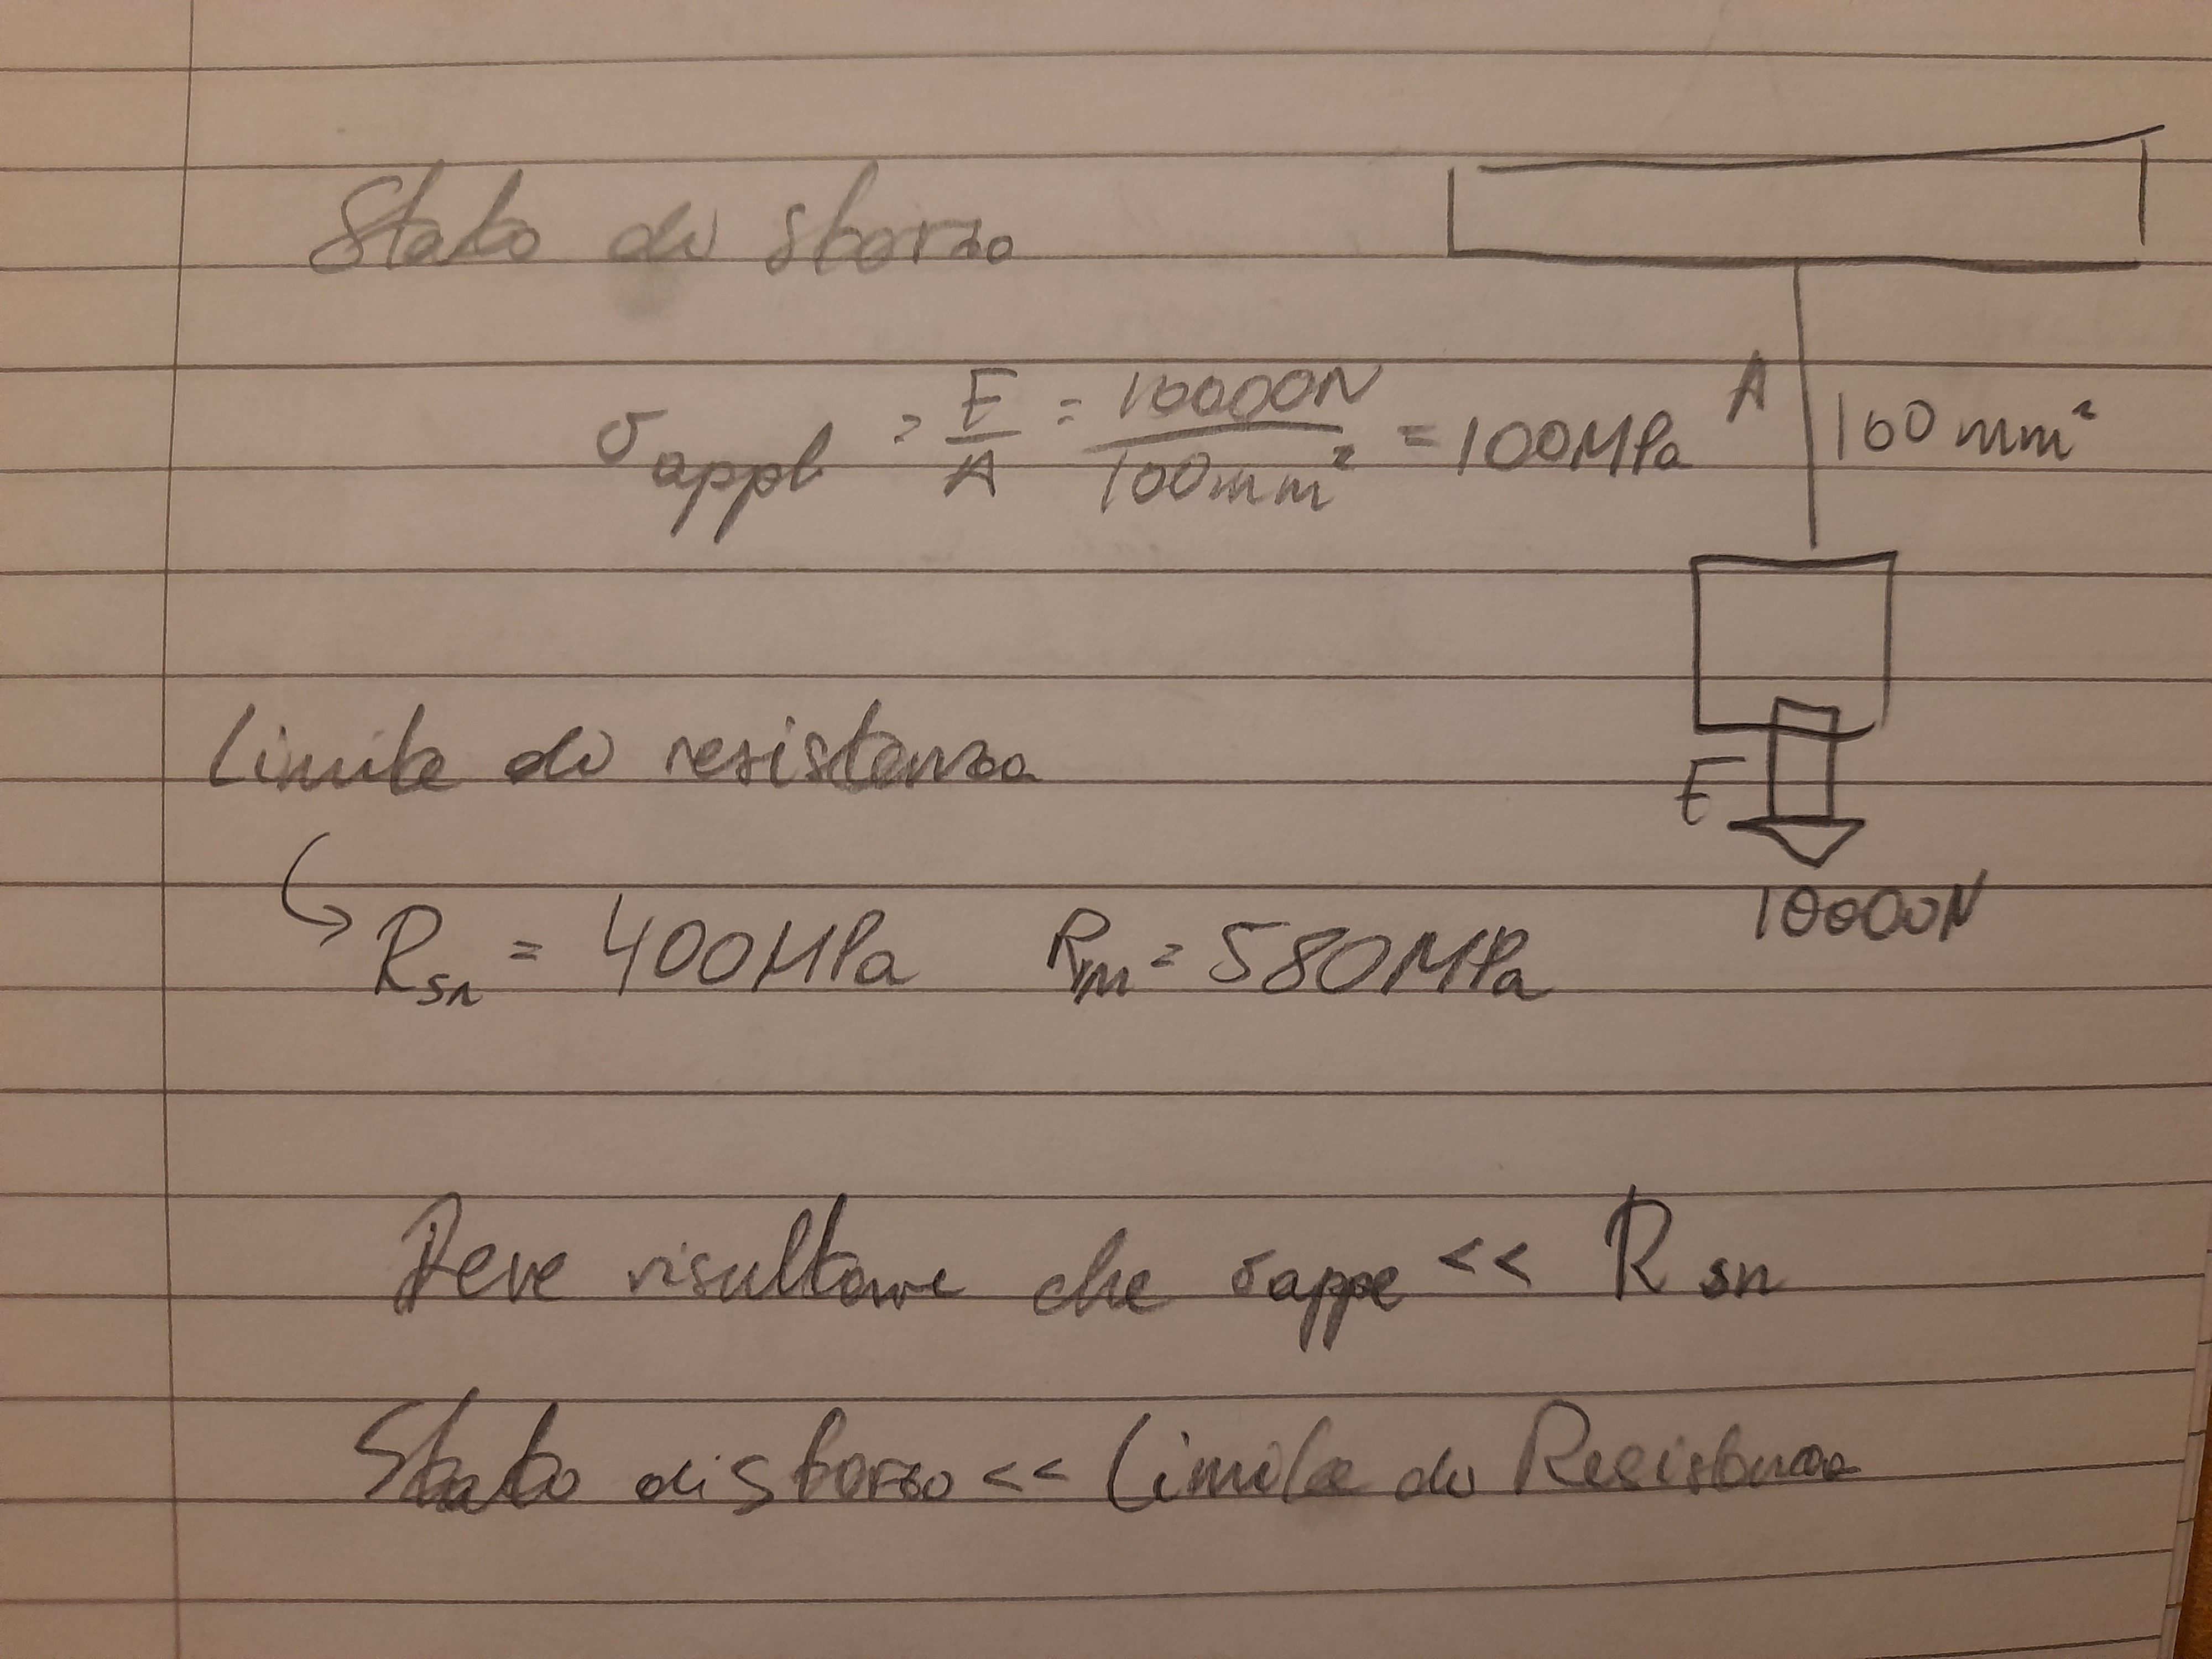
\includegraphics[width=.85\linewidth]{Esempio di Esercizio Limite di Sforzo.jpg}
            \end{figure}
            La prova di trazione \'e di rricavare i numeri per esser sicuri che il materiale sia giusto per il caso a cui sta venendo sottoposto.
        \subsection{Coefficiente di sicurezza}
            Il coefficiente di sicurezza \'e la proporzione tra il limite della resistenza e lo stato di sforzo, questo numero \'e tenuto normalmente intorno a 2. Il numero quantifica quanta quanta volte deve esser multiplicato lo sforzo perch\'e si arrivi al limite di resistenza. Usando questo numero si pu\'o vedere se si pu\'o diminuire la sezione o aumentare i cavi. 
    \section{Lezione 7 - Le Prove di Durezza di Materiale Metallici}
        Durezza $\rightarrow$ resistenza a penetrazione
        \subsection{Durezza per Improntatura}
                La resistenza di un materiale alla penetrazione di un corpo di durezza superiore e di definita geometria. Il carico si applica lentamente in direzione perpendicolare alla superficie.
                \begin{itemize}
                    \item Brinell
                    \item Vickers
                    \item Rockwell
                \end{itemize}
                \subsubsection{Prova di Brinell}
                    La prova di Brinell consiste nel prendere una sfera di acciaio duro, o carburo di tungsteno e applicare un carico perpendicolare alla superfice del materiale che si vuole improntare.
                    \begin{figure}[!h]
                        \centering
                        \includegraphics[width=.85\linewidth]{Grafico Durezza Brinell.png}
                    \end{figure}
                    Si trova la media dei due diametri (paralleli al piano) di penetrazione perch\'e la forza forse non \'e distribuita perfettamento.\\ \\
                    La durezza Brinell [HB]:
                    \begin{figure}[!h]
                        \centering
                        \includegraphics[width=.85\linewidth]{Equazione per Durezza Brinell.png}
                    \end{figure}
                    Il penetratore nella prova di Brinell \'e una sfera in acciaio duro o carburo di tungsteno di diametro D = 10mm (il diametro pu\'o cambiare ma \'e pi\'u comunemente 10mm) il e forza di F = 29400N(3000kg). La prova come molte altre cose nella ingegneria \'e normata.\\ \\
                    Per esguire la prova Brinell bisogna fissare c = $\frac{F}{D^2}$, carico in N per mm di diametro. Nel caso si usano i chili la formula \'e c = $0.102\frac{F}{D^2}$. Queste formule esistono perch\'e per diversi materiali e diversi diametri bisogna applicare diverse forze.\\ \\
                    Il rapporto tra F e D deve esser la costante c, perch\'e quando si fissa c si fissa anche $\alpha$ che \'e l'angolo del triangolo creato dalla base di d.
                    \begin{figure}[!h]
                        \centering
                        \includegraphics[width=.85\linewidth]{Tabella per Valore c Prova Brinell.png}
                    \end{figure}
                    Fissando c si assicura che c'\'e troppa o troppa poca penetrazione. Per ci\'o si prova a fissare c per ottende un angola $\alpha$ tra 106$^o$ e 152$^o$, ma l'angolo ottimo \'e di 136$^o$. Imponendo l'angolo equivale a imporre anche la proporzione tra il diametro della fossa e il diametro del penetratore, tra 0,24 e 0,60 con un valore preferito di 0,375.\\ \\
                    \begin{figure}[!h]
                        \centering
                        \includegraphics[width=.85\linewidth]{Diagramma alpha per Prova Brinell.png}
                    \end{figure}
                    La distribuzione delle forze \'e meglio se permette la creazione di una calotta con le dimensioni giuste. Se si penetra troppo si perdono molti componenti di forza trasversali. Se invece di penetra troppo poco si perdono componenti di forza penetranti. Per rendere il risultato ripetibile si usa la proporzione c.\\ \\
                    La durezza Brinell (HB) ha correllazione con la resistenza meccanica/massima degli acciai.
                    \begin{figure}[!h]
                        \centering
                        \includegraphics[width=.85\linewidth]{Diagramma di Rm con Durezza Brinell nell'acciaio.png}
                    \end{figure}
                \subsubsection{Durezza Vickers}
                    \begin{figure}[!h]
                        \centering
                        \includegraphics[width=.85\linewidth]{Diagramma per la Prova Vickers.png}
                    \end{figure}
                    La prova di Vickers ha lo stesso scopo della prova di Brinell.
                    La equazione per la Durezza Vickers(HV) \'e $HV = \frac{F}{S}$, cio\'e gli stessi parametri.\\ \\
                    Il penetratore della prova di Vickers \'e diverso dalla prova di Brinell. Nella prova di Vickers il penetratore \'e una piramdie di diamante a base quadrata con aongolo al vertico di 136$^o$. Il carico pu\'o essere qualunque perch\'e la il penetratore permette risultati proporzionali, per ci\'o i risultati possono essere confrontati a diversi carichi. \'E anche possibile trestare materiali molto duri perch\'e il penetratore \'e di diamante.\\ \\
                    La durezza Vickers a causa della forma del penetratore non ha lo stesso vantaggio della Durezza di Brinell.\\ \\
                    La prova di Vickers crea calotta piccol che \'e buono se si vuole testa materiali omogenei per\'o causa problemi con materiali eterogenei perch\'e il risultato pu\'o cambiare basato su dove \'e testato. Per ci\'o la prova Brinell \'e usata quando il materiale \'e eterogeneo, perch\'e lascia una impronta grande.\\ \\
                    La durezza Brinell \'e circa uguale alla durezza Vickers (HB $\cong$ 0,95 HV). \\ \\
                    Le prova Brinell e Vickers danno quasi sempre 3 cifre negli acciai.
                \subsubsection{Prova Rockwell}
                    La prova Rockwell \'e formata da 7 prove diverse pe\'o guarderemo solo 2 di quest prove. La prova Rockwell C $\rightarrow$ Cone $\rightarrow$ HRC, e la prova Rockwell B $\rightarrow$ Ball $\rightarrow$ HRB.
                    \begin{figure}[!h]
                        \centering
                        \includegraphics[width=.85\linewidth]{Diagrammi per le Prova di Durezza Rockwell.png}
                        \caption{Per HRC e HRB, P \'e il carico applicato e h \'e la profondit\'a della calotta.}
                    \end{figure}
                     Generalmente pi\'u \'e duro un materiale pi\'u e resistente. all'affondamento. \\ \\
                    Anche se la prova Rockwell \'e simile alla Vickers e Brinell, guarda qualcosa di diverso dall Vickers e Brinell per determine la durezza, per ci\'o non sono correllate.\\ \\
                    HRB opera a 90kg, mentre la HRC \'e a 140kg.
                    \begin{figure}[!h]
                        \centering
                        \includegraphics[width=.85\linewidth]{Diagramma di Affondamento per la Prova di Rockwell.png}
                    \end{figure}
                    \begin{figure}[!h]
                        \centering
                        \includegraphics[width=.85\linewidth]{Tabella per le Prova di Rockwell.png}
                    \end{figure}
                \newpage
                \subsubsection{Prova di Durezza Portatile}
                    \begin{figure}[!h]
                        \centering
                        \includegraphics[width=.85\linewidth]{Diagramma di Prova di Durezza Portatile.png}
                    \end{figure}
                    Le forza HB sono proporzionali ai loro diametri basata sulla stessa forza. Questo \'e un modo di prova la durezza di un materiale, perche sapendo la durezza della piastra di riferimento, si pu\'o derivare la durezza del pezzo.
            \subsection{Resilienza e resistenza alla frattura fragile (Resistenza agli impatti)}
                Fattori che contribuiscono ad indurre fratture fragile:
                \begin{enumerate}
                    \item Velocit\'a di Applicazione del Carico
                    \item Temperatura
                    \item Presenza di intagli (sforzo equitriassiale)
                \end{enumerate}
                Se non ci sono le sollecitazione a taglio non c'\'e scorrimento, c'\'e la rottura fragile.
                \subsubsection{Prova Charpy}
                    La prova Charpy consiste nel far cadere una massa su un provino di materiale con tagli diversi.\\ \\
                    \newpage
                    \begin{figure}[!h]
                        \centering
                        \includegraphics[width=.85\linewidth]{Diagramma per le Prove Charpy.png}
                    \end{figure}
                    \begin{figure}[!h]
                        \centering
                        \includegraphics[width=.85\linewidth]{Diagramma per il metodo di Prova Charpy.png}
                    \end{figure}
                    \begin{figure}[!h]
                        \centering
                        \includegraphics[width=.85\linewidth]{Diagramma e equazione per la prova charpy.png}
                    \end{figure}
                    Durante la prova di trova che a certe temperature il materiale pu\'o resistere impatti di certe energie. \\ \\
                    \newpage
                    I materiali hanno una soglia di accettabilit\'a per la loro fragilit\'a, questo valore \'e normato e viene trovato usando al curva di transizione.
                    \begin{figure}[!h]
                        \centering
                        \includegraphics[width=.85\linewidth]{Diagramma per la Resilienza in confronto alla temperatura di prova.png}
                    \end{figure}
                    Svolgendo molte prova a varie temperature si ottiene un grafico, che fa vedere una curva del cambio in resilienza con in confronto al cambio di temperature di prova. Con questo si pu\'o determinare un valore termico $T_transizione$ dove il materiale va da essere fragile a tenace. \newpage
                    \begin{figure}[!h]
                        \centering
                        \includegraphics[width=.85\linewidth]{Diagramma sulla Curva di Transizione nella Resilienza contro temperatura di prova.png}
                    \end{figure}
                    Per determine la temperature di transizione si usa la equazione:
                    \begin{gather*}
                        (KV_\text{max} + KV_\text{min})/2 \approx x (J) \\
                        \text{A} x (J) T_\text{transizione} \approx y^o C
                    \end{gather*}
    \section{Lezione 8 - Continuazione dell'ultima lezione e Diagrammi di Stato}
        Ad alta temperature i provini che sono sottoposto alle prove di resilienza si deformano di pi\'u di quando hanno temperatura pi\'u bassa, la differenza in deformazione rappresenta il cambio da fragilit\'a alla tenacit\'a.
        \newpage
        \subsection{3 Tipi di Curve di Resilienza}
            \begin{figure}[!h]
                \centering
                \includegraphics[width=.85\linewidth]{Tipi di Curve di Prova di Resilienza.png}
            \end{figure}
            L'obbiettivo della prova di resilienza \'e di trovare la temperature di transizione.
            Un materiale che non ha temperature di transizione \'e favorito perch\'e agisce a modo tenace a tutte le temperature e \'e pi\'u facile da utilizzare. Se ce l'ha la temperatura di transizione \'e meglio una $T_\text{tr}$ pi\'u bassa che pi\'u bassa.
            \newpage
            \begin{figure}[!h]
                \centering
                \includegraphics[width=.85\linewidth]{Tipi di Curve di Prova di Resilienza basato sul tipo di reticolo.png}
            \end{figure}
            La temperature di transizione \'e connessa al tipo di reticolo che il metallo ha, per esempio i reticoli C.F.C non hanno $T_tr$ invece i reticolo C.C.C ce l'hanno.
        \subsection{Effetto della dimensione del grano}
           \begin{figure}[!h]
                \centering
                \includegraphics[width=.85\linewidth]{Correllazione tra temperatura di transizione e dimensione del grano.png}
            \end{figure}
        \subsection{Effetto del Carbonio}
            Il carbonio "avvelena" il matierale e diminuisce la resilienza.
            \begin{figure}[!h]
                \centering
                \includegraphics[width=.85\linewidth]{Effetto del carbonio sulla resilienza del materiale.png}
            \end{figure}
            \subsubsection{Effetto del Manganese}
                Il manganese \'e meglio per la resilienza, impede le rottura fragile. Quest'effetto lo fa anche il nickel, ma ad una certa $\%$ \'e persa, perch\'e ad alta $\%$ la struttura del Ni cambia naturalmente al C.F.C
        \subsection{Diagrammi di Stato dei materiali metallici}
            \underline{Definizione} - Un sistema chimico (un sistema chiuso fisicamento dal mondo esterno) - Parte di una matiera separate dal fuori da una soglia. \\
            \subsubsection{Sistema chimico omogeneo}
                Se il sistema ha composizione chimica uguale ad ogni punto nel sistema, lo stato \'e uguale ad ogni punto di stesso P e T.
            \subsubsection{Sistema chiuso eterogeno}
                Ogni sistema che non soddisfa tutte e tre le condizioni per un sistema omogeneo.
        \subsection{Fase}
            Una fase \'e una porzione omogenea in un sistema eterogeneo.
            \begin{figure}[!h]
                \centering
                \includegraphics[width=.85\linewidth]{Esempio delle fasi in un sistema chiuso dei composti.png}
            \end{figure}
            Ci sono 2 fasi omogene se C in tutte e due hanno stessa T,P e composizione chimica.
        \subsection{Diagramma di Fase dell'acqua}
            \begin{figure}[!h]
                \centering
                \includegraphics[width=.85\linewidth]{Diagramma di stato dell'acqua.png}
            \end{figure}
            Le zone tra le line sono le zone fasiche, le linea sono le sezioni bifasiche, manche il punto triplo \'e l'unico punto dove tutte e tre le fasi sono presenti. Questo \'e un diagramma tipico per materiali sono metallici.
        \subsection{Diagramma di stato di Fe}
            \begin{figure}[!h]
                \centering
                \includegraphics[width=.85\linewidth]{Diagramma di stato del Ferro puro.png}
            \end{figure}
            Anche i metalli hanno diagrammi di fase, dove le fasi possono includere zone di diverse strutture reticolari.
        \subsection{Teorema di Gibbs}
            \begin{equation*}
                V = C_i + M - F
            \end{equation*}
            \begin{itemize}
                \item V = varianza (numero di gradi di libert\'a
                \item C$_i$ = componenti chimici indipendenti (C$_t$ - r)
                \item M = fattori fisici effettivi
                \item F = fasi
            \end{itemize}
            La varianza rappresenta quante direzioni nel diagramma di fasi si pu\'o muovere e rimanere nella stessa fase.
            \begin{figure}[!h]
                \centering
                \includegraphics[width=.85\linewidth]{Punti di Variazione nel diagramma di stato dell'acqua.png}
            \end{figure}
            \begin{figure}[!h]
                \centering
                \includegraphics[width=.85\linewidth]{Esempio di variazione di un sistema chiuso.png}
            \end{figure}
        \subsection{Stato Binario}
            Sistema omogeneo tra due agenti chimici.\\
            Come uno diagramma di stato per\'o invece di pressione fa vedre la correllazione tral a composizione chimica (A-B) e la temperatura. Cio\'e rappresenta la fasi all'equilibrio del sistema A-B al variare della temperatura. Questo viene chiamato diagramma di stato.\\ \\
           \begin{figure}[ht]
                \centering
                \includegraphics[width=.85\linewidth]{Cambio nella curva di raffreddamento in un sistema completamente miscibilie esemplare.png}
            \end{figure}
            Qualunque sostanza pura ha un cambio di stato a temepratura unica.\\
            Con le leghe, come visto nel diagramma, le leghe hanno 2 temperature importanti. Perch\'e c'\'e un inclinaggio non \'e una linea dritta.\\
            Le leghe metalliche si solidificano in un intervallo di temperature. I due punti sono dove inizia e finisce la solificazione.
            \begin{figure}[!h]
                \centering
                \includegraphics[width=.85\linewidth]{Zone di stato in un diagramma di stato per due leghe compleamente miscibili.png}
            \end{figure}
            Diagramma di fase per in materiali perfettamente miscibili, cio\'e sono completamente solubili quando solidi e liquidi.
    \section{Lezione 9 - Diagramma di Completa Miscibilit\'a}
        \begin{figure}[!h]
            \centering
            \includegraphics[width=.85\linewidth]{Zone di stato in un diagramma di stato per due leghe compleamente miscibili - Parte 2.png}
        \end{figure}
        \begin{figure}[!h]
            \centering
            \includegraphics[width=.85\linewidth]{Indice delle indicazioni di sistema e fasi nei diagrammi di stato.png}
        \end{figure}
        \begin{figure}[!h]
            \centering
            \includegraphics[width=.85\linewidth]{Sistem 30pc B completamente miscibile.png}
        \end{figure}
        La solidificazione dei metalli \'e sempre attraverso la nucleazione a crescimento, questo \'e important perch\'e sar\'a un fattore importante su come si former\'a diverse leghe. Nel esempio della completa mischibilit\'a un mischio di A e B si forma nei grani a crescimento. \\ \\
        \begin{figure}[!h]
            \centering
            \includegraphics[width=.85\linewidth]{Cambio nel sistema completamente miscibile a 30pc B.png}
        \end{figure}
        Con un cambio di concentrazione, quando \'e tutto liquido \'e omogeneo e quando \'e tutto solido \'e omogeneo.
        Le concentrazioni delle fasi cambiano perch\'e un metallo di solidifica pi\'u velocemente dell'altro, per\'o nel sistema effettivo la concentrazione non cambio sono nelle fasi se stesse. Se si volesse separare i metalli si pu\'o rimuovere i solidi quando il metallo non \'e ancora solidificato completamente, visto che le fasi hanno concentrazioni diverse dal sistema il solido non avr\'a la stessa concentrazione del sistema ma una diversa, quindi lentamente si pu\'o rimuovere un metallo.
        \subsection{Variazione nel diagramma di stato binario}
            \begin{figure}[!h]
                \centering
                \includegraphics[width=.85\linewidth]{Esempio di variazione in diagramma di stato binario .png}
            \end{figure}
            Nel punto 1 e 2, la varianza \'e 2, questo \'e perch\'e tutti e due sono monofasici, mentre l'area centrale a una varianza di 1 perch\'e sono bifasici.
            \newpage
        \subsection{Traiettorie di raffradamento}
            Abbiamo gi\'a parlato di traiettorie di raffreddamento, per\'o ora parleramedo di perch\'e sono cos\'i.
            \begin{figure}[!h]
                \centering
                \includegraphics[width=.85\linewidth]{Spiegazione per il cambio di inclinazione nelle traiettorie di raffraddamento.png}
            \end{figure}
            La pendenza della traiettoriaa cambia perch\'e c vuole pi\'u energia per cambiare fasi. La pendenza prima e dopo la solidificazione (cio\'e agli stati completamente liquidi e solidi ) la pendenza non \'e uguale ma simile, per\'o visto che il raffreddamento ci mette molto tempo il tempo \'e rappresentato da $log(t)$ e quindi la pendanza \'e effettivamente uguale. Le leghe non si solidificano e una temperatura costante, ma ad un intervallo di temperature, questo spiega perch\'e bisogna aggiungere/togliere il calore latente.
        \subsection{Calcolare la Quantit\'a delle fasi / Regola della leva}
            La regola della leva \'e un metodo per determine le quantit\'a delle fasi di una lega, durante la solidificazione o liquifazione, ma anche quano una lega non sta cambiando stato.
            \newpage
            \begin{figure}[!h]
                \centering
                \includegraphics[width=.85\linewidth]{Spiegazione della regola della leva per un sistema con metalli con puri.png}
            \end{figure}
            Usando la equazione $\frac{\text{Segmento Opposto}}{\text{Segmento Totale}}$ si pu\'o determinare le quantit\'a nel sistema. Se si prendono linea che vanno dai punti alla asse orizzontale si pu\'o trovare anche la composizione chimica di tutte e due le fasi.
        \subsection{Esercizio tipico}
            \begin{figure}[!h]
                \centering
                \includegraphics[width=.85\linewidth]{Esempi di esercizi nei diagramma di stato binario.png}
            \end{figure}
        \newpage
        \subsection{Diagramma di Stato Binario di Completa immiscibilit\'a allo stato solido}
            \begin{figure}[!h]
                \centering
                \includegraphics[width=.85\linewidth]{Diagramma di stato binario di completa immiscibilita allo stato solido per una soluzione basilare.png}
            \end{figure}
            Le due vericali sono i metalli puri di tutte e due gli elementi, le due line oblique sono chiamate linee liquidus, mentre la linea orizzontale \'e chimata la orizzontale eutettica.
            I campi monofasici sono:
            \begin{itemize}
                \item Liquido
                \item Verticale Sinistra
                \item Verticale Destra
            \end{itemize}
            La lega in alcuni punti ha una temperatura di fusion di pi\'u bassa della temperatura di fusion di tutti e due i metalli, la legha che si fonda alla temperatura pi\'u bassa \'e chiamata leghe eutettica, e la concentrazione dove appere cambio tra ogni combinazione di metalli.
            \subsubsection{Curve di Raffreddamento di leghe completamente immiscibili a stato solido}
                Una cosa importante da ricordarsi \'e che la pendenza non \'e proporzionale alla varianza.\\ \\
                \begin{figure}[ht]
                    \centering
                    \includegraphics[width=.85\linewidth]{Esempio di curve di raffreddamento di una soluzione di metallo puro in un sistema completamente immiscibile.png}
                \end{figure}
                \begin{figure}[ht]
                    \centering
                    \includegraphics[width=.85\linewidth]{Curva di Raffreddamento per una lega eutettica esemplare.png}
                \end{figure}
                La curva di raffreddamento della lega eutettica \'e molto simile a quella dei metalli puri, questo \'e perch\'e nella lega eutettica non occorre un a transizione tra fasi per\'o solo una solidificazione normale come i metalli puri.
                \begin{figure}[!h]
                    \centering
                    \includegraphics[width=.85\linewidth]{Curva di Raffreddamento per una lega non-eutettica esemplare.png}
                \end{figure}
                Le leghe non eutettiche hanno un intervallo di temperature per la transizione di fasi, per\'o quando raggiungono l'orizzontale eutettico anche loro hanno una varianza di 0.
                \newpage
        \subsection{Leghe Eutettiche}
            \begin{figure}[!h]
                \centering
                \includegraphics[width=.85\linewidth]{Diagramma di cambio strutturale in un sistema completamente immiscibile binario - Parte 1.png}
            \end{figure}
            Le leghe eutettiche formano strutture lamellari non miscielate. \\ \\
            La cosa pi\'u importante \'e che quando un a lega raggiunge la temperatura eutettica nel sistema:\\ \\
            \paragraph{Il liquido, tutto il liquido e solo il liquido che arriva alla temperatura eutettica si trasforma nel costituente strutturale eutettico a lamelle alterante delle due fasi solide.}
            Cio\'e tutto il liquido nel sistema si trasforma in una struttura a lamelle alternate. Questo \'e vero anche per le leghe non eutettiche che \'e la ragione perch\'e anche la loro curva di raffreddamento diventa orizzontale.
            \begin{figure}[!h]
                \centering
                \includegraphics[width=.85\linewidth]{Struttura esemplare di grani cristallini lamellari, per un sistema di metalli completamente immiscibili.png}
            \end{figure}
            Le lamelle sono completamente non miscelate.
            \begin{figure}[!h]
                \centering
                \includegraphics[width=.85\linewidth]{Cambio di struttura prima e dopo la temperature eutettica in un sistema esemplare di metalli completamente immiscibili.png}
            \end{figure}
            Le leghe eutettiche si formano per nucleazione a crescimento e si formano ad un passo costante per ci\'o si pu\'o determine la quantita a diversi punti nel tempo.
            \begin{figure}[! h]
                \centering
                \includegraphics[width=.85\linewidth]{Cambio nelle fasi prima e dopo la temperatura eutettica in un sistema completamente miscibilie esemplare.png}
            \end{figure}
             La struttura lamellare \'e composta da 2 fasi ma un tipo di struttura. Per ci\'o si pu\'o anche determinare la quantita di diverse fasi a tempi diversi.
             \begin{figure}[!h]
                \centering
                \includegraphics[width=.85\linewidth]{Carcolo di fase e costituenti di una lega eutettica esemplare in un sistema di metalli completamente immiscibili.png}
            \end{figure}
             La cosa importante da sapere \'e che le fasi non sono la stessa cosa dei costituenti strutturali, le fasi sono le diverse combinazioni di metalli miscelati, invece i costituenti strutturali sono i tipi di struttura che compongono il sistema i costituenti strutturali possono essere fasi o possono essere combinazioni di fasi. In questo caso ci sono 2 metalli non miscilati per ci\'o due fasi, per\'o queste due fasi creano una struttura lamellare che compone il sistema completamente.
             \begin{figure}[!h]
                \centering
                \includegraphics[width=.85\linewidth]{Cambio di struttura tra dopo eutettica e temperature ambiente in un sistema esemplare di metalli completamente immiscibili.png}
            \end{figure}
             Nelle leghe eutettiche a completa immiscibilit\'a non c'\'e cambio nella struttura di una lega a alla temperatura eutettica e un lega a temperatura ambiente.
    \newpage
    \section{Lezione 10 - Continuazione delle Leghe Eutettiche, le leghe Ipoeutettiche e i diagrammi di parziali solubilit\'a}
        La caratteristica definitiva delle leghe eutettiche a completa immiscibilit\'a \'e che la loro struttura \'e comopletamente lamella a lamella alternate, questo \'e eterogeno non omogeneo.\\ \\
        I grani lamellari sono pi\'u resistenti dei grani omogenei perch\'e i reticoli di A e B sono diversi quindi le dislocazioni non hanno spazio per viaggiare, questo rende il materiale meno deformabile e i\'u resistente.\\ \\
        Studiare il diagramma di stato aiuta a capire le propritet\'a una lega avr\'a.
        \subsection{Lega Ipoeutettica}
            Una lega ipoeutettica \'e una leghe con una contrazione del metallo B minore di quello richiesto per una lega eutettica.
            \begin{figure}[h!]
                \centering
                \includegraphics[width=.85\linewidth]{Diagramma di stato di lega ipoeutettica e traiettoria di solidificazione.png}
            \end{figure}
            \begin{figure}[h!]
                \centering
                \includegraphics[width=.85\linewidth]{Cambio nella stuttura nella lega ipoeutettica da T0 a TEU.png}
            \end{figure}
            Nella lega ipoeutettica la fa A inizia a formare grani omogenei di fase A che crescono fino all'orizzontale eutettico.
            \begin{figure}[h!]
                \centering
                \includegraphics[width=.85\linewidth]{Cambio nella stuttura nella lega ipoeutettica attraverso TEU.png}
            \end{figure}
            Attraversando l'orizzontale il liquido e tutto il liquido forma grani lamellari di fasi A e B, incapsulando i grani omogenei nei grani lamellari.\\ \\
            La maggior parte delle leghe di fonderia sono leghe eutettiche, perch\'e si fondono a temperature pi\'u basse dei metalli stessi e creano la struttura lamellare che \'e pi\'u resistente.\\ \\
            \begin{figure}[h!]
                \centering
                \includegraphics[width=.85\linewidth]{Calcoli per Fasi e Costituenti nella lega ipoeutettica prima di TEU.png}
            \end{figure}
            \'E importante distinguere le fasi dai costituenti strutturali.
            \begin{figure}[h!]
                \centering
                \includegraphics[width=.85\linewidth]{Calcoli per Fasi e Costituenti nella lega ipoeutettica dopo di TEU.png}
            \end{figure}
            Il rapporto della concentrazione delle fasi nella struttura lamellare, \'e lo stesso rapporto della concentrazione all'eutettico.\\ \\
            Per trova concentrazione a meta tempo di solidificazione aggiungere concentrazione a t$_1$ e t$_2$ e dividere per 2.
        \subsection{Lega Ipereutettica}
            La lega ipereutettica \'e come la lega ipoeutettica per\'o i grani omogenei saranno di B non A.
            \newpage
        \subsection{Limiti di Solubilit\'a}
            \begin{figure}[h!]
                \centering
                \includegraphics[width=.85\linewidth]{Esempio di Limite di Solubilita in un sistema acqua zucchero.png}
            \end{figure}
            Questo \'e un esempio della solubilit\'a usando lo zucchero e l'acqua. La curva nel grafico \'e il limite di solubilit\'a dopo che si passa (aumentando la concentrazione di zucchero, una parte dello zucchero inizia a precipitare come solido perch\'e l'acque non pu\'o pi\'u tenere cos\'i tanto zucchero. Se la temperatura di abbassa, il limite di solubilit\'a si abbassa, e quindi l'acqua non tiene quando zucchero come poteva e per ci\'o inizia a smiscelare e pi\'u acque  Questo concetto \'e analogo nei metalli.
        \subsection{Diagramma di stato di parziale solubilit\'a}
            \begin{figure}[h!]
                \centering
                \includegraphics[width=.85\linewidth]{Diagramma di stato di parziale solubilita esemplare.png}
            \end{figure}
            Nei diagrammi di parziale miscibilit\'a ci sono aree dove i metalli sono miscibilie con l'un 'altro a stato liquido e solido. Queste are possono esser sopra e sotto la temperature eutettica, per\'o l'eutettica tutto il liquido diventa struttura lamella di A o $\alpha$ e B o $\beta$. Se il limite di solubilit\'a (le line diagonali o curve) diminuisce le fasi smiscelano l'un l'altro.
        \newpage
        \subsection{Lega Ipoeutettica a solubilit\'a parziale allo stato solido}
            \begin{figure}[h!]
                \centering
                \includegraphics[width=.85\linewidth]{Diagramma di stato di parziale solubilita per lega ipoeutettica e traiettoria di raffreddamento .png}
            \end{figure}
            Tra T$_1$ e T$_3$ il materiale \'e come ogni altra lega ipoeutettica oltre il fatto che si forma $\alpha$ e non A. I punto angoloso nella traittoria di raffreddamento occorre perch\'e la transizione \'e da solido a solido per ci\'o l'inclinazione cambio, ma non \'e ovvia nel diagramma perch\'e si usa log(t). Dopo T$_3$ \'e tutto solido.\\
            \newpage
            \begin{figure}[h!]
                \centering
                \includegraphics[width=.85\linewidth]{Diagramma di stato di parziale solubilita per lega ipoeutettica e cambio di struttura tra T0 e T4.png}
            \end{figure}
            $\alpha$ \'e una fase omogenea quindi crea grani con un reticolo omogeneo. A T$_5$ si incontra il limite di solubilit\'a (cio\'e il limite di solubilit\'a di B in $\beta$) questo causa $\alpha$ a smiscelare $\beta$.\\
            \begin{figure}[h!]
                \centering
                \includegraphics[width=.85\linewidth]{Diagramma di stato di parziale solubilita per lega ipoeutettica e smiscielamento tra T5 e TAMB.png}
            \end{figure}
            $\beta$ viene smiscielato in forma di placchette a bordo grano dei grani omogenei di $\alpha$. Questo cambio occorre tra T$^-_\text{EU}$ e T$_\text{AMB}$.\\
            \begin{figure}[h!]
                \centering
                \includegraphics[width=.65\linewidth]{Calcoli per Fasi e Costituenti nella lega ipoeutettica per metalli parzialmente miscibili a TAMB.png}
                \caption{Calcolo delle fasi e costituenti a T$_\text{AMB}$}
            \end{figure}
            Diagrammi analoghi per le leghe ipereutettiche a parziali miscibilit\'a a stato solido.\\
    \section{Lezione 11 - Leghe Ausiliarie, ipoeutettiche fuori dal campo $\alpha$ e il peritettico}
        \subsection{La lega ausliaria}
            \begin{figure}[h!]
                \centering
                \includegraphics[width=.85\linewidth]{Diagramma di stato di parziale solubilita per lega ipoeutettica dopo campo a e traiettoria.png}
            \end{figure}
            La durata di t, l'arresto termico, raggiunge il minimo pi\'u vicino si \'e alla lega ausiliaria. La struttura si forma con gli stessi principi delle altre leghe. Quest\'a \'e la lega che smiscela di pi\'u.\\ \\
            \begin{figure}[h!]
                \centering
                \includegraphics[width=.70\linewidth]{Calcolo per la lega ausiliaria per materiali parzialmente miscibile.png}
            \end{figure}
            Questa lega \'e importante perch\'e ha il massimo di smiscelamento, e visto che il cambio nello smiscelamento \'e proporzionale al cambio di concentrazione per ci\'o la si pu\'o usare per calcolare lo smiscelamento in altre leghe nel caso che non sia chiaro.
        \subsection{Lega eutettica per materiali parzialmente miscibili}
            \begin{figure}[h!]
                \centering
                \includegraphics[width=.85\linewidth]{Diagramma di stato per lega eutettica tra materiali parzialmente miscibili e traiettoria.png}
            \end{figure}
            \begin{figure}[h!]
                \centering
                \includegraphics[width=.85\linewidth]{Diagramma di stato di parziale solubilita per lega ipoeutettica dopo campo a e cambio di struttura.png}
            \end{figure}
            La lega eutettica si forma come prima, per\'o invece di esser formata da cristalli lamellari di A e B, \'e formata da cristalli lamellari di $\alpha$ e $\beta$ \\ \\
            La lega cambia con il cambio solubilit\'a. Le fasi $\alpha$ e $\beta$ smiscelano l'un l'altro, per ci\'o tutti e due cambio per\'o perch\'e smiscelano quantita diverse e sono in proporzioni diverse, nei calcoli sembrer\'a che sono uno sta smiscelando.
            \begin{figure}[h!]
                \centering
                \includegraphics[width=.85\linewidth]{Diagramma di smiscelamento tra fasi parzialmente miscibili.png}
            \end{figure}
        \subsection{Lega Ipoeutettica fuori dai campi parziale miscibilit\'a}
            Questa lega \'e lo stesso ipoeutettica, ma perch\'e non entra nel campo $\alpha$ o $\beta$ la struttra non \'e composta completamente da grani omogenei.\\ \\
            \begin{figure}[h!]
                \centering
                \includegraphics[width=.8\linewidth]{Diagramma per la lega ipoeutettica fuori dal campo alpha con curva di raffreddamento.png}
            \end{figure}
            \begin{figure}[h!]
                \centering
                \includegraphics[width=.8\linewidth]{Diagramma per la lega ipoeutettica fuori dal campo alpha e cambio di struttura prima di TEU.png}
            \end{figure}
            \begin{figure}[h!]
                \centering
                \includegraphics[width=.8\linewidth]{Diagramma per la lega ipoeutettica fuori dal campo alpha e cambio di struttura dopo TEU.png}
            \end{figure}
            \newpage
            Come detto prima, il liquido, tutto il liquido e solo il liquido che arriva all'orizzontale eutettico crea cristalli lamellari.\\ \\
            \begin{figure}[h!]
                \centering
                \includegraphics[width=.85\linewidth]{Calcolo per la lega ipoeutettica fuori dal campo prima di TEU.png}
            \end{figure}
            \begin{figure}[h!]
                \centering
                \includegraphics[width=.85\linewidth]{Calcolo per la lega ipoeutettica fuori dal campo dopo TEU.png}
            \end{figure}
            Come si vede la fase $\alpha$ aumenta perch\'e la si formano i cristalli lamellari che contengono se stessi della fase $\alpha$.\\ \\
            \begin{figure}[h!]
                \centering
                \includegraphics[width=.8\linewidth]{Calcolo per lega ipoeutettica fuori dal campo a meta tempo di arresto.png}
            \end{figure}
            Di nuovo, le transizioni sono lineari per ci\'o se si vuole trovare le concentrazioni a met\'a tempo si pu\'o trovare la media.\\ \\
            \subsubsection{Cambio nella struttura tra T$^-_\text{EU}$ e T$_\text{AMB}$}
                Come in ogni altra lega in questo esempio, tra l'orizzontale eutettico e la temperatura ambiente c'\'e lo smiscelamento.\\ \\
                \begin{figure}[h!]
                    \centering
                    \includegraphics[width=.8\linewidth]{Diagramma di smiscelamento per lega ipoeutettica fuori da campo .png}
                \end{figure}
                Sia $\alpha$ che $\beta$ smiscelano, in questo caso c'\'e pi\'u $\alpha$ quindi smiscela di pi\'u. Visto che ci sono sia grani omogenei di $\alpha$ e cristalli lamellari, tutti e due smiscelano quindi si formano placchette di $\beta$ e la concentrazione nelle strutture lamellari cambia.\\ \\
                \begin{figure}[h!]
                    \centering
                    \includegraphics[width=.8\linewidth]{Calcolo per lega ipoeutettica fuori dal campo a TAMB senza risposte.png}
                \end{figure}
                Come detto prima, ci sono dei casi dove \'e difficile calcolare la concentraizone dei costitutenti lamellari, probabilmente perch\'e la concentrazione di una fase cambio in due costituenti e non solo uno. Per questo si usa la lega ausilieria, e si fa una stima usando il cambio di concentrazione della lega.\\ \\
                \begin{figure}[h!]
                    \centering
                    \includegraphics[width=.8\linewidth]{Spiegazione per l'uso della lega ausiliaria per trovare smiscelamento in casi estranei.png}
                \end{figure}
                \begin{figure}[h!]
                    \centering
                    \includegraphics[width=.8\linewidth]{Calcolo per lega ipoeutettica fuori dal campo a TAMB con risposta.png}
                \end{figure}
        \subsection{Lega Ipereutettica}
            Come in ogni altro caso la lega ipereutettica \'e un caso analogo alla lega ipoetettica ma $\alpha$ e $\beta$ sono cambiati.
        \subsection{La trasformazione peritettica}
            \begin{figure}[h!]
                \centering
                \includegraphics[width=.85\linewidth]{Diagramma di stato per leghe peritettiche esemplari.png}
            \end{figure}
            Questo \'e un diagramma tipico di una trasformazione peritettica, la lega a X \'e chiamata la lega peritettica. Per notare la differenza tra eutettica e il peritettico si pu\'o dire che nell'eutettico le "orecchie" sono in su, mentre nel peritettico sono un "orecchio" \'e in su.\\ \\
            La trasformazione peritettica comporta SEMPRE la formazione di grani cristallini omogenei, e mai lamellari. Nel caso della trasformazione peritettica, perch\'e non si formano cristalli lamellari, le fasi coincidono sempre con le strutture.\\ \\
            \newpage
            \begin{figure}[h!]
                \centering
                \includegraphics[width=.85\linewidth]{Casi di leghe nei diagrammi di stato per leghe peritettiche.png}
            \end{figure}
            \subsubsection{Lega Peritettica}
                \begin{figure}[h!]
                    \centering
                    \includegraphics[width=.85\linewidth]{Diagramma di stato e traietoria di raffreddamento per lega peritettica.png}
                \end{figure}
                Nella reazione peritettica, $\alpha$ reagisce con il liquido per formare $\beta$, \'e come una reazione chimica.\\ \\
            \subsubsection{Lega Ipoperitettica}
                \begin{figure}[h!]
                    \centering
                    \includegraphics[width=.85\linewidth]{Diagramma di stato e traietoria di raffreddamento per lega ipoperitettica.png}
                \end{figure}
                In questo caso c'\'e troppo $\alpha$ quindi grani di $\alpha$ e $\beta$ coesistono.\\ \\
            \subsubsection{Lega Iperperitettica}
                \begin{figure}[h!]
                    \centering
                    \includegraphics[width=.85\linewidth]{Diagramma di stato e traietoria di raffreddamento per lega iperperitettica.png}
                \end{figure}
                Dopo il peritettico c'\'e ancora liquido che \'e la ragion per il cambio di pendenza e l'arresto di raffreddamento, e poi si raffredda normalmente.\\ \\
        \subsection{Nomenclatura dei tipi di diagrammi di stato.}
            \begin{figure}[h!]
                \centering
                \includegraphics[width=.85\linewidth]{L11 - Diagramma per la nomenclatura di tipi di diagrammi di stato.png}
            \end{figure}
            Se non c'\'e liquido ma c'\'e $\gamma$ e il nome cambia. La fase $\gamma$ non cambia come di trasforma la struttura, cambio solo la traiettoria di raffreddamento\\ \\
    \newpage

    \section{PSA}
        Dalla lezione 12 alla lezione 14 ci saranno un bel po di foto a causa della natura e complicatezza del materiale dipinto.
    \section{Lezione 12 - Liquido vs. $\gamma$, Esempi di esercizi e diagramma ferro-carbonio}
        \subsection{Liquido vs. $\gamma$}
            \begin{figure}[h!]
                \centering
                \includegraphics[width=.85\linewidth]{L12 - Diagramma con gamma e Liquido.png}
            \end{figure}
            In quest'esempio esiste una fase liquida e una fase $\gamma$. La orizzontale \'e detta eutettoidica perche c'\'e gamma invece del liquido, ma come se ci fosse il liquido, $\gamma$ si trasforma in $\alpha$ e $\beta$ e quando si arriva alla temperature eutettoidica, $\gamma$, tutto $\gamma$ e solo $\gamma$ si trasforma in cristalli lamellari. La struttura di $\gamma$ \'e a grani omogenei.
        \subsection{Esempi di esercizi}
            In alcuni casi pu\'o essere che i diagrammi sono connessi, e esistono dei materiali intermedi tra i due materiali principali, questi caso portrebbero apparire nell'esame.
            \begin{figure}[h!]
                \centering
                \includegraphics[width=.75\linewidth]{L12 - Esempio di esercizio possibileper l'esame.png}
            \end{figure}
        \newpage
        \subsection{Cosa utile da ricordare per l'esame}
            Se si traccia una linea orizzontale su un diagramma di stato, linea passa tra fasi alternanti tra monofasico e bifasico. Bisogna ricordarsi che se c'\'e una linea verticale nel mezzo quella conta come un campo monofasico.
        \subsection{Diagramma di stato ferro-carbonio}
            \begin{figure}[h!]
                \centering
                \includegraphics[width=.85\linewidth]{L12 - Diagramma Fe-C non simplificato.png}
            \end{figure}
            Questo \'e il diagramma di stato tra il ferro e il carbonio, bisogna sapere le temperature e concentrazioni. Una cosa interessante \'e che il diagramma finisce a 6,69$\%$ di carbonio perch\'e dopo questo punto il carbonio non riesce pi\'u a miscelarsi con il ferro.\\ \\
            Gli acciai sono le leghe che vanno da un infinitesimo di carbonio alla lega ausiliare di 2,11$\%$ di carbonio. Mentre la ghisa va dal 2,11$\%$ di carbonio al 6,69$\%$ di carbonio.\\ \\
            La ragione per le dimensione enorme del campo $\gamma$ in confronto ai campo $\alpha$ e $\sigma$ \'e che la fase $\gamma$ accetta meglio gli atomi interstiziali perch\'e ha lacune pi\'u grandi. 
            \subsubsection{Simplificazione del diagramma di stato Fe-C}
                \begin{figure}[h!]
                    \centering
                    \includegraphics[width=.85\linewidth]{L12 - Diagramma Fe-C non simplificato.png}
                \end{figure}
                Le simplificazioni occorono perch\'e rendono i calcoli pi\'u semplici. Le due simplificazioni sono la compressione della zona $\alpha$ per renderla sono una linea, e il rimuovimento del campo $\sigma$ perch\'e in molti cosi sar\'a inutile sapere che esiste. 
                \begin{figure}[h!]
                    \centering
                    \includegraphics[width=.85\linewidth]{L12 - Diagramma Fe-C simplificato.png}
                \end{figure}
            \newpage
            \subsubsection{Casi per l'esame}
                \begin{figure}[h!]
                    \centering
                    \includegraphics[width=.85\linewidth]{L12 - Diagramma Fe-C Casi di Esercizi per L'Esame.png}
                \end{figure}
                Questi sono i 4 casi possibili per l'esame nella seconda domanda.
            \subsubsection{Diagramma per il ferro puro}
                \begin{figure}[h!]
                    \centering
                    \includegraphics[width=.85\linewidth]{L12 - Diagramma Fe-C diagramma e traiettoria per ferro puro.png}
                \end{figure}
                Il ferro puro durante il raffreddamento crea cristalli omogenei di fase $\gamma$ e poi a T$_3$ per nucleazione a crescimento dal bordo grano si formano grani omogenei di $\alpha$. Passando l'eutettoidico non ha effetto perch\'e non c'\'e pi\'u $\gamma$.
                \begin{figure}[h!]
                    \centering
                    \includegraphics[width=.85\linewidth]{L12 - Diagramma Fe-C - Ferro Puro - Cambio di Struttura.png}
                \end{figure}
                \begin{figure}[h!]
                    \centering
                    \includegraphics[width=.85\linewidth]{L12 - Diagramma Fe-C - Ferro Puro - Cambio di Struttura 2.png}
                \end{figure}
            \newpage
            \subsection{Convenzioni di Nomenclatura}
                Per rendere pi\'u facile la descrizione, i grani omogenei di fase $\gamma$ vengono chiamati Austenite, mentre i grani omogenei di fase $\alpha$ vengono chiamati Ferrite.
        \subsection{Lega Eutettoidica (0,77$\%$)}
            \begin{figure}[h!]
                \centering
                \includegraphics[width=.85\linewidth]{L12 - Diagramma Fe-C - 0,77C - Diagramma e Traiettoria.png}
            \end{figure}
            \begin{figure}[h!]
                \centering
                \includegraphics[width=.85\linewidth]{L12 - Diagramma Fe-C - 0,77C - Cambio di Struttura 1.png}
            \end{figure}
            Fino all'orizzontale eutettoidico la struttura non \'e diversa dell'eutettico, cambio sono come si forma perch\'e deve fare una transizione termica.
            \begin{figure}[h!]
                \centering
                \includegraphics[width=.85\linewidth]{L12 - Diagramma Fe-C - 0,77C - Cambio di Struttura 2.png}
            \end{figure}
            Attraversando l'eutettoiodico, tutto gamma diventa una struttura a cristalli lamellari di $\alpha$ e Fe$_3$C.
            \begin{figure}[h!]
                \centering
                \includegraphics[width=.85\linewidth]{L12 - Diagramma Fe-C - 0,77C - Calcolo all'eutettoidico.png}
            \end{figure}
            \begin{figure}[h!]
                \centering
                \begin{subfigure}{.45\linewidth}
                    \includegraphics[width=\linewidth]{L12 - Diagramma Fe-C - 0,77C - Cambio costituenti.png}
                \end{subfigure}
                \begin{subfigure}{.45\linewidth}
                    \includegraphics[width=\linewidth]{L12 - Diagramma Fe-C - 0,77C - Cambio fasi.png}
                \end{subfigure}
            \end{figure}
            Dopo l'eutettoidico la struttura non cambio neache andando gi\'u finoa a T$_\text{AMB}$.
        \subsection{Convenzioni di Nomenclatura}
            I grani cristallini lamellari di $\alpha$ e Fe$_3$C sono noti come Perlite.
        \newpage
        \subsection{Lega Ipoeutettoidica (Caso A) (0,40$\%$)}
            \begin{figure}[h!]
                \centering
                \includegraphics[width=.85\linewidth]{L12 - Diagramma Fe-C - 0,40C - Diagramma e Traiettoria.png}
            \end{figure}
            \begin{figure}[h!]
                \centering
                \includegraphics[width=.85\linewidth]{L12 - Diagramma Fe-C - 0,40C - Cambio di Struttura 1.png}
            \end{figure}
            Di nuovo prima dell'eutettoidico, oltre al tempo di formazione, il sistema di forma come un metallo puro.\\ \\
            \newpage
            \begin{figure}[h!]
                \centering
                \includegraphics[width=.8\linewidth]{L12 - Diagramma Fe-C - 0,40C - Cambio di Struttura 2.png}
            \end{figure}
            Appena si passa la linea del solidus, la fase $\gamma$ inizia a smiscelare cristalli omogenei di $\alpha$ a bordo grano.
            \begin{figure}[h!]
                \centering
                \includegraphics[width=.8\linewidth]{L12 - Diagramma Fe-C - 0,40C - Cambio di Struttura 3.png}
            \end{figure}
            Appena si attraversa l'eutettoidico tutto il $\gamma$ che \'e rimasto cambia si trasforma in perlite.
            \begin{figure}[h!]
                \centering
                \includegraphics[width=.8\linewidth]{L12 - Diagramma Fe-C - 0,40C - Calcolo all'eutettoidico.png}
            \end{figure}
            \begin{figure}[h!]
                \centering
                \includegraphics[width=.8\linewidth]{L12 - Diagramma Fe-C - 0,40C - Fasi e Costituenti all'eutettoidico.png}
            \end{figure}
            Di nuovo dopo l'eutettoidico e anche fino a T$_\text{AMB}$ la struttura non cambia.
            \begin{figure}[h!]
                \centering
                \includegraphics[width=.8\linewidth]{L12 - Diagramma Fe-C - 0,40C - Cambio di Struttura 4.png}
            \end{figure}
            \subsubsection{Generalizzazione}
                Tra $0\%<C<0,77\%$ la lega Fe-C \'e a temperatura ambiente formata da Ferrite e Perlite, in quantit\'a dipendenti dalla concentrazione del carbonio.
    \section{Lezione 13 - Lega Ipereutettoidica (Caso B - 0,77$\%$ < C < 2,11$\%$)}
        Questa sar\'a un'p\'o pi\'u corta perch\'e durante la lezione il Prof.Boniardi ha fatto vedere degli esempi di domande che ci saranno durante l'esame.
        \subsection{Esempio di lega a 1$\%$ C}
            \begin{figure}[h!]
                \centering
                \includegraphics[width=.8\linewidth]{L13 - Curva di Stato per Accaio a C = 1.png}
            \end{figure}
            \begin{figure}[h!]
                \centering
                \includegraphics[width=.8\linewidth]{L13 - Cambio di struttura prima del eutettoidico.png}
            \end{figure}
            \begin{figure}
                \centering
                \begin{subfigure}[h!]{0.6\linewidth}
                    \includegraphics[width=\linewidth]{L13 - Cambio di struttura durante lo smiscelamento della cementite a C = 1.png}
                \end{subfigure}
                \begin{subfigure}[h!]{0.3\linewidth}
                    \includegraphics[width=\linewidth]{L13 - Struttura del sistema dopo l'eutettoidico.png}
                \end{subfigure}
            \end{figure}
            \newpage
            T$_4$ \'e 100$\%$ fase $\gamma$ cio\'e 100$\%$ cristalli omogenei di fase $\gamma$ aka Austenite
            \subsubsection{Convenzioni di Nomenclatura}
                La struttura formata da lamelle di $\alpha$ e Fe$_3$C ci chiama Perlite\\
                Mentre le placchette di Fe$_3$C vengono chiamate Cementite secondaria (scritto Cementite II).
            \begin{figure}[h!]
                \centering
                \includegraphics[width=.8\linewidth]{L13 - Fe-C 1C Calcolo fasi e costituenti.png}
            \end{figure}
            \begin{figure}[h!]
                \centering
                \includegraphics[width=.8\linewidth]{L13 - Fe-C 1=C Diagrammi fasi e costituenti.png}
            \end{figure}
            Di nuovo tra dopo l'eutettoidico e T$_{AMB}$ non c'\'e cambio nei componenti strutturali
        \newpage
        \subsection{Lega Ausiliare ($\%C$ = 2,11$\%$)}
            \begin{figure}[h!]
                \centering
                \includegraphics[width=.8\linewidth]{L13 - Fe-C 2,11C Diagramma di stato e linea di raffreddamento.png}
            \end{figure}
            Alle estremita dell'orizzontale d'arresto, significa che alla cementite viene dato il tempo massimo per smiscelare.\\
            \begin{figure}[h!]
                \centering
                \includegraphics[width=.85\linewidth]{L13 - Cambio di struttura per C = 2,11 prima del eutettico.png}
            \end{figure}
            \begin{figure}
                \centering
                \begin{subfigure}[h!]{.6\linewidth}
                    \includegraphics[width=\linewidth]{L13 - Cambio di struttura per C = 2,11 dopo l'eutettico e prima del eutettoidico.png}
                \end{subfigure}
                \begin{subfigure}[h!]{.3\linewidth}
                    \includegraphics[width=\linewidth]{L13 - Cambio di struttura dopo l'eutettoidico.png}
                \end{subfigure}
            \end{figure}
            \begin{figure}[h!]
                \centering
                \includegraphics[width=.85\linewidth]{L13 - Fe-C 2,11C Calcolo fase e costituenti prima e dopo l'eutettoidico.png}
            \end{figure}
            \begin{figure}[h!]
                \centering
                \includegraphics[width=.8\linewidth]{L13 - Fe-C 2,11C Diagrammi di fase e costituenti prima e dopo l'eutettoidico.png}
            \end{figure}
        \newpage
            Di nuovo non c'\'e cambio tra eutettoidico e T$_{AMB}$\\
        \newpage
        \subsection{Generallizazione dell'ipereutettoidico}
            In generale qualucque lega Fe-C con composizione iperetuttoidica cio\'e 0,77$\%$ < C < 2,11$\%$ \'e composta a T$_{AMB}$ da Cementite e Perlite. Con un massimo di 22,6$\%$ di cementite.   
    
    \newpage
    \section{Lezione 14 - Le strutture degli acciai (composti Fe-C con $\%$C < 2,11 $\%$), Lega Eutettica, Lega Ipoeutettica e Lega Ipereutettica}
        \subsection{Le strutture degli acciai}
            L'analisi delle strutture dei diversi acciai occorre attraverso un processo di analisi micrografica. Un campione dell'acciaio viene lucidato, questo significa che quando la luce viene posta sul campione e un immagine \'e fatta, le parti lisce e perpendicolari all'oggetto che sta facendo la foto vengono viste come aree bianche, mentre le imperfezioni vengono viste come aree grigie o nere.\\
            \subsubsection{Strutture}
                \begin{figure}[h!]
                    \centering
                    \includegraphics[width=.65\linewidth]{L14 - Austenite.png}
                \end{figure}
                L'Austenite \'e composta da grani omogenei di fase $\gamma$ e sotto il microscopio \'e si vede come sopra.\\\newpage
                \begin{figure}[h!]
                    \centering
                    \includegraphics[width=.65\linewidth]{L14 - Ferrite.png}
                \end{figure}
                La ferrite invece \'e composta da grani omogenei di fase $\alpha$ e sotto il microscopio viene vista come sopra.\\
                \begin{figure}[h!]
                    \centering
                    \includegraphics[width=.65\linewidth]{L14 - Perlite e Cementite.png}
                \end{figure}
                La perlite \'e formata la lamelle di fase $\alpha$ e Fe$_3$C, sotto il microscopio di vedono le lamelle della perlite, nella stessa immagine si vedono anche delle fasce bianche che sono la cementite II, cio\'e Fe$_3$C.\\
                \begin{enumerate}
                    \item Eutettoidico - 100$\%$ Perlite
                    \item Ipoeutettoidico - Ferrite e Perlite
                    \item Ipereutettoidico - Perlite e Cementite
                \end{enumerate}
            \subsubsection{Punti Critici}
                \begin{figure}[h!]
                    \centering
                    \includegraphics[width=.8\linewidth]{L14 - Diagramma Punti Critici.png}
                \end{figure}
                I punti critici sono I punti dove diversi composti iniziano e finiscono a formarsi. Questi punti critici nei diagrammi si stato vengono rappresentati dalla linee di transizione. A$_3$ \'e la linea di inizio dove la Ferrite inizia a formarsi indipendentemente, e A$_{CM}$ \'e dove la cementite viene formata indipendentemente, mentre la linea A$_1$ \'e dove la ferrite e cementite iniziano a formarsi allo stesso tempo cio\'e quando inizia a formarsi la Perlite.\\

            \subsubsection{Elementi di lega e l'effetto sul diagramma}
                I diagrammi di stato sono diagrammi ideali dove ci sono solo Fe e C. L'acciaio per\'o pu\'o avere elementi alleganti che cambiano il diagramma di stato. Ci sono due classi si elementi alleganti, gl'elementi Austenitizzanti che espandono l'area dell'Austenite e Stringono il campo $\alpha$ o gl'elementi Ferritizzanti che allargano il campo $\alpha$ e stringono il campo dell'Austenite.\\
            \newpage
                \begin{figure}[h!]
                    \centering
                    \includegraphics[width=.8\linewidth]{L14 - Diagramma elementi austenitizzanti e ferritizzanti.png}
                \end{figure}
                Le diverse leghe possono esser usate per propriet\'a oltre la resistenze, e alcuni materiali vanno bene che siano pi\'u deformabili o fragili perch\'e anche loro hanno il loro uso.\\
                \begin{figure}[h!]
                    \centering
                    \includegraphics[width=.8\linewidth]{L14 - Diagramma Austenitizzato e Ferritizzato con + 10pc.png}
                \end{figure}
                Questo \'e come di ottengono immagini delle strutture dell'acciai che dovrebbero esistere solo a centinaia o migliaia di gradi.\\
        \newpage
        \subsection{Lega Eutettica (C = 4,3$\%$)}
            \begin{figure}[h!]
                \centering
                \includegraphics[width=.7\linewidth]{L14 - C = 4,3 Diagramma di Stato e Traiettoria di Raffreddamento.png}
            \end{figure}
            \begin{figure}[h!]
                \centering
                \includegraphics[width=.7\linewidth]{L14 - C = 4,3 Strutture 1148+ a 1148-.png}
            \end{figure}
            All'eutettico globulare, nel ferro all'eutettico, non si forma una struttura lamellare, ma invece si formano grani di fase $\gamma$ che inglobano grani di Fe$_3$C. Questi grani non sono chiamati Austenite perch\'e non sono omogenei, invece sono noti come Ledeburite.\\
            \begin{figure}[h!]
                \centering
                \includegraphics[width=.7\linewidth]{L14 - C = 4,3 Calcolo 1148-.png}
            \end{figure}
            \begin{figure}[h!]
                \centering
                \includegraphics[width=.7\linewidth]{L14 - C = 4,3 Diagrammi Fasi e Costituenti 1148+ a 1148-.png}
            \end{figure}
            \begin{figure}[h!]
                \centering
                \includegraphics[width=.7\linewidth]{L14 - C = 4,3 Strutture 1148- a 727+.png}
            \end{figure}
            \newpage
            La fase $\gamma$ smiscela Fe$_3$C e si chiama lo stesso Ledeburite.\\
            
            \begin{figure}[h!]
                \centering
                \includegraphics[width=.7\linewidth]{L14 - C = 4,3 Calcolo 727+.png}
            \end{figure}
            \newpage
            Dopo l'eutettoidico la fase $\gamma$, sono la fase $\gamma$ e tutte la fase $\gamma$ si trasforma in perlite, questa nuova struttura viene chiamata ledeburite trasformata.\\
            \begin{figure}[h!]
                \centering
                \includegraphics[width=.7\linewidth]{L14 - C = 4,3 Strutture 727+ a 727-.png}
            \end{figure}
            \begin{figure}[h!]
                \centering
                \includegraphics[width=.7\linewidth]{L14 - C = 4,3 Calcolo 727-.png}
            \end{figure}
            Di nuovo da dopo 'eutettoidico e T$_{AMB}$ la strututra non cambia.\\

        \subsection{Lega Ipoeutettica (C = 2,5$\%$) - Caso C}
            \begin{figure}[h!]
                \centering
                \includegraphics[width=.7\linewidth]{L14 - C = 2,5 Diagramma di Stato e Traiettoria di Raffreddamento.png}
            \end{figure}
            \begin{figure}
                \centering
                \begin{subfigure}[h!]{.55\linewidth}
                    \includegraphics[width=\linewidth]{L14 - C = 2,5 Strutture Prima di 1148+.png}
                \end{subfigure}
                \begin{subfigure}[h!]{.3\linewidth}
                    \includegraphics[width=\linewidth]{L14 - C = 2,5 Strutture a 1148-.png}
                \end{subfigure}
            \end{figure}
            \newpage
            Dopo l'eutettico ci sono le sturtture di Austenite e Ledeburite.\\
            \begin{figure}[h!]
                \centering
                \includegraphics[width=.7\linewidth]{L14 - C = 2,5 Calcolo tra 1148+ a 1148-.png}
            \end{figure}
            \begin{figure}[h!]
                \centering
                \includegraphics[width=.7\linewidth]{L14 - C = 2,5 Diagrammi Fase e Costituenti da 1148+ a 1148-.png}
            \end{figure}
            \begin{figure}[h!]
                \centering
                \includegraphics[width=.7\linewidth]{L14 - C = 2,5 Strutture tra 1148- a 727+.png}
            \end{figure}
            \begin{figure}[h!]
                \centering
                \includegraphics[width=.7\linewidth]{L14 - C = 2,5 Calcolo a 727+.png}
            \end{figure}
            \begin{figure}[h!]
                \centering
                \includegraphics[width=.7\linewidth]{L14 - C = 2,5 Calcolo a 727+ con Lega Ausiliare.png}
            \end{figure}
            \newpage
            Per questo calcolo bisogna usare la lega Ausiliaria per trova la quantita di ogni costituenti strutturale, vedendo all'Ausiliaria c'era inizialmente 100$\%$ austenite mentre ora c'\'e solo 82,2$\%$ e si forma proporzionalmente. \\
            \begin{figure}[h!]
                \centering
                \includegraphics[width=.7\linewidth]{L14 - C = 2,5 Strutture da 727+ a 727-.png}
            \end{figure}
            \begin{figure}[h!]
                \centering
                \includegraphics[width=.7\linewidth]{L14 - C = 2,5 Calcolo a 727-.png}
            \end{figure}
            \begin{figure}[h!]
                \centering
                \includegraphics[width=.7\linewidth]{L14 - C = 2,5 Diagrammi Fase e Costituenti da 727+ a 727-.png}
            \end{figure}
            \newpage
            Di nuovo la struttura non cambio dopo l'eutettoidico.\\
        \subsection{Lega Ipereutettica (C = 5$\%$)}
            \begin{figure}[h!]
                \centering
                \includegraphics[width=.8\linewidth]{L14 - C = 5 Diagramma di Stato e Traiettoria di Raffreddamento.png}
            \end{figure}
            \begin{figure}[h!]
                \centering
                \includegraphics[width=.7\linewidth]{L14 - C = 5 Strutture prima di 1148+.png}
                \caption{Il punto di domanda non ]'e perche non sappiamo la struttura \'e perch\'e non si spiega molto bene come fa ad esser stabile.}
            \end{figure}
            \begin{figure}[h!]
                \centering
                \includegraphics[width=.55\linewidth]{L14 - C = 5 Strutture da 1148+ a 1148-.png}
            \end{figure}
            \begin{figure}[h!]
                \centering
                \includegraphics[width=.8\linewidth]{L14 - C = 5 Calcolo da 1148+ a 1148-.png}
            \end{figure}
            \begin{figure}[h!]
                \centering
                \includegraphics[width=.8\linewidth]{L14 - C = 5 Diagrammi di Fasi e Costituenti da 1148+ a 1148-.png}
            \end{figure}
            \begin{figure}[h!]
                \centering
                \includegraphics[width=.7\linewidth]{L14 - C = 5 Strutture da 1148- a 727+.png}
                \caption{Solo i globuli aumentano in dimensione}
            \end{figure}
            \begin{figure}[h!]
                \centering
                \includegraphics[width=.8\linewidth]{L14 - C = 5 Calcolo da 1148- a 727+.png}
            \end{figure}
             \begin{figure}[h!]
                \centering
                \includegraphics[width=.7\linewidth]{L14 - C = 5 Strutture da 727+ a 727-.png}
            \end{figure}
             \begin{figure}[h!]
                \centering
                \includegraphics[width=.8\linewidth]{L14 - C = 5 Calcolo a 727-.png}
            \end{figure}
             \begin{figure}[h!]
                \centering
                \includegraphics[width=.7\linewidth]{L14 - C = 5 Diagrammi di Fasi e Costituenti da 727+ a 727-.png}
            \end{figure}

    \section{Lezione 15 - Curve di Trasformazione isoterme (TTT - Time Temperature Transformation)}
        L'acciaio pu\'o esser sottoposta a cicli di trattamento termico. Un ciclo termico \'e caratterizzato da un riscaldamento, un mantenimento alla temperatura finale e un raffreddamento.\\
        \begin{figure}[h!]
            \centering
            \includegraphics[width=.7\linewidth]{Metallurgia/L15 - Diagramma ciclo termico ideale.png}
        \end{figure}
        \newpage
        Il diagramma di stato di un materiale \'e rappresentativo del raffreddamento pi\'u lento, invece se l'acciaio fosse sottoposto ad un trattamento di raffreddamento pi\'u brusco, c'\'e la possibilit\'a che il trasformazione di $\gamma$ non darebbe lo stesso risultato del trattamento pi\'u lento.\\
        \subsection{Curve TTT}
            \begin{figure}[h!]
                \centering
                \includegraphics[width=.75\linewidth]{Metallurgia/L15 - Ciclo TTT.png}
            \end{figure}
            Il mantenimento alle temperature sopra i punti critici e in fatto in modo per permettere la formazione dell'austenite perch\'e per effettuare la trasformazione ci vuole tempo. I punti critici sono I punti di trasformazione di Austenite, che nel diagramma di stato sono A$_1$, A$_3$ e A$_{cm}$ e gli stessi simboli verrano usati anche in questi casi.\\
            Il TTT convilge un riscaldamento, mantenimento, raffreddamento e mantenimento ad una temperatura, poi durante questo mantenimento l'Austenite inizia a trasformarsi e ri formano diverse strutture. Il punto dove la trasformazione inizia e finisce viene segnato e messo in un grafico.\\
            \newpage
            \begin{figure}[h!]
                \centering
                \includegraphics[width=.75\linewidth]{Metallurgia/L15 - TTT con cerchi e croci.png}
            \end{figure}
            L'esperienza di Bain \'e il nome dato quando le linee formate da questo processo sono tracciate e analizzate.  Si trovano diversi campi, per primo il campo della perlite (nel caso di C = 0,77$\%$, ferrite e cementite anche a diverse concentrazioni) che \'e sopra la gobba dalla C formata dal grafico, mentre il campo della Bainite \'e sotto la gobba. Le linee horizzontali rappresentato l'inizio e la fine della formazione della Martensite, che sono sempre damercate da M$_s$ per Martensite start e a volte M$_f$ per Martensite finish.\\
            \begin{figure}[h!]
                \centering
                \includegraphics[width=.75\linewidth]{Metallurgia/L15 - TTT per C77.png}
            \end{figure}
            La Marteniste avveine durante il raffreddmanento brusco del metallo non a t = cost, quindi se M$_s$ \'e stata passata ci sar\'a sempre almeno un'p\'o di martensite. Se M$_f$ \'e passata ci sar\'a solo la Martensite, mentre se si passa M$_s$ ma non M$_f$ con un'p\'o di tempo si former\'a anche della Bainite.
            La Martensite e Bainite sono considerate strutture di non-equilibrio mentre la ferrite e perlite sono strutture di equilibrio.\\
            Essendo strutture di non-equilibrio la Bainite e Martensite non appargon sul diagramma di stato.
        \subsection{Esempio di Curva TTT per un acciaio ipoeutettoidico}
            \begin{figure}[h!]
                \centering
                \includegraphics[width=.7\linewidth]{Metallurgia/L15 - TTT Ipoeutettoidico.png}
            \end{figure}
            Per ogni acciaio esiste una e una sola curva di raffreddamento.
            Se un acciaio di mantiene ad una temperatura appena sotto A$_1$ non si forma solo perlite ma si forma anche la ferrite (cementite nel caso i acciai ipereutettoidici)
        \subsection{Curva TTT vera per acciaio C45}
            \begin{figure}[h!]
                \centering
                \includegraphics[width=.7\linewidth]{Metallurgia/L15 - Cicli esemplare C45.png}
            \end{figure}
            In questo esempio si possono vedere diverse cose. Per primo I numeri accanto alla curva rappresentano la quantita finale della struttura alla fine del trattamento, cio\'e 25$\%$ di ferrite e 75$\%$Perlite a 600$^o$C. Mentre i numeri dentro i cerchi sono la durezza del materiale, dato che sono solo due numeri sono HRC per\'o se fossero 3 sarebbe HV, si pu\'o notare che pi\'u un metallo \'e lontano dall'equilibrio pi\'u \'e duro.
            
        
    
\end{document}